\chapter{Princip postačitelnosti, podmíněnosti, věrohodnosti, zastavovací pravidlo sekvenčního principu, vztahy.}
Uvedené principy nejsou věty, ale něco, co chceme, aby platilo ve statistické procedůře (zatím ne Bayesovské).
\begin{description}
	\item[SUFFICIENCY princip:] Máme experiment $\mathcal{E}$ závislý na~$\t$, pozorování $x,y$ a~nechť je v~$\mathcal{E}$ k~dispozici postačující statistika $T$ (PS). Víme-li, že $T(x)=T(y)$,~chceme, aby závěry o~$\t$ na~základě $x$ nebo $y$ byly shodné. ($T$ je PS, pokud rozdělení $X|T(X)=t$ nezávisí na~$\t$).
	
	\item[LIKELIHOOD princip:] Informace o~$\t$ nesená $x$ je zcela obsažena ve~věrohodnostní funkci $L(\t)=f_\X(\textbf{x},\t)$. Navíc, pokud máme pozorování $x_1$ v experimentu $\mathcal{E}_1$ a~$x_2$ v~experimentu $\mathcal{E}_2$ taková, že 
	$$ L_1(\t|x_1)=c L_2(\t|x_2),\quad\forall\t\in\Theta,$$
	pak chceme, aby závěry o~parametru $\t$ v~obou experimentech byly shodné. Označíme to $\mathrm{Ev}(\mathcal{E}_1,x_1)=\mathrm{Ev}(\mathcal{E}_2,x_2)$ (Ev jako Evidence). 
	
	\item[CONDITIONALITY princip:] Tento princip se od prvních dvou liší tím, že chceme, aby něco platilo pro všechna potenciálně naměřená data. Nechť máme dostupné $\mathcal{E}_1,\mathcal{E}_2$. Definujeme $\mathcal{E}^*$ experiment tak, že vybereme náhodně mezi~$\mathcal{E}_1 \vee \mathcal{E}_2$ a~v~tom vybraném naměříme $x_j,~j=1\vee 2$. Chceme, aby $\Ev\big(\mathcal{E}^*,(j,x_j)\big)=\Ev(\mathcal{E}_j,x_j),~\forall j,\forall x_j$. V prvním (složeném) experimentu tedy zaznamenáváme $j\in\{0,1\}$ jako index experimentu a $x_j$ jako naměřenou hodnotu a chceme, aby závěr ze složeného experimentu byl stejný, jako kdyby nevybraný experiment vůbec neexistoval.
	\item[STOPPING rule:] Máme posloupnost experimentů $\mathcal{E}_1,\mathcal{E}_2,...$ a zastavovací pravidlo $\tau$, které zastavuje posloupnost v~bodě $\mathcal{E}_n$. Jsou naměřeny $\textbf{x}=\big( x_1^{\mathcal{E}_1},x_2^{\mathcal{E}_2},...,x_n^{\mathcal{E}_n} \big)$. Chceme, aby $\Ev\big( \{ \mathcal{E}_1,...,\mathcal{E}_n,\tau \},\textbf{x} \big)$ závisela na~$\tau$ pouze prostřednictvím $\textbf{x}$, tzn. $$\Ev\big( \{ \mathcal{E}_1,...,\mathcal{E}_n,\tau_1 \},\textbf{x} \big)=\Ev\big( \{ \mathcal{E}_1,...,\mathcal{E}_n,\tau_2 \},\textbf{x} \big),~\forall \textbf{x}.$$
	\item[BAYESOVSKÝ princip:] Taková procedura, která využívá k~rozhodnutí o~parametru $\t$ aposteriorní hustotu $\pi(\t|\textbf{x})=\frac{f_\X(\textbf{x}|\t)\cdot\pi(\t)}{\int f_\X(\textbf{x}|\t)\cdot\pi(\t) \d\t}$, např. $\widehat{\t}_\mathrm{B}=''\EE{\pi(\t,\textbf{x})}''=\E^\pi(\t)$.
\end{description}

\begin{example}
	Mějme $\mathcal{E}_j..x_j\in\Ran(X_j)$, kde $X_j\sim f(x_j,\t),~\forall j\in 1,2,...$. Teoreticky můžeme jít až do~nekonečna, ale někdy chceme experiment zastavit, abychom mohli vyhodnotit data. Definujeme tedy $\tau$ jako zastavení v~bodě $n$, pokud $$\textbf{x}:=(x_1,...,x_n)\in\Ran(X_1)\times\Ran(X_2)\times...\times\Ran(X_n)\equal{ozn}\Aa_n.$$ Platí, že
	$$ L(\t|\textbf{x})\equal{id}\Big(\prod f_{X_j}(x_j,\t) \Big)\cdot I_{\Aa_n}(\textbf{x})\equal{non~id}f(x_1|\t)f(x_2|x_1,\t)...f(x_n|x_1,x_2,...,x_{n-1},\t)I_{\Aa_n}(\textbf{x}).$$
	Vidíme, že $L(\t|\textbf{x})$ nezávisí na zastavovacím pravidlu $\tau$ přímo, ale pouze prostřednictvím $\textbf{x}$. Tedy pokud platí $L$ princip, potom platí i $SR$ princip.
\end{example}
\begin{example}
	Máme TV seriál. Označme $\t\in[0,1]$ jako sledovanost daného dílu. Bylo zjištěno, že 9 diváků seriál sledují a~3 nikoliv (to jsou naše data). Problém je, že nevíme, jakým způsobem byla data naměřena. 
	\begin{description}
		\item[$\mathcal{E}_\mathrm{I}:$] vybráno $n=12$ lidí, otestováno, získána data (9DIV,3NEDIV). Máme tedy náhodnou veličinu $X$ jako počet diváků z~$n=12$ nezávislých opakování. Z~toho plyne, že $X\sim \Bi(12,\t)$. Máme napozorováno $X(\omega)=x=9$.
		\item[$\mathcal{E}_\mathrm{II}:$] vybíráme $x$ osob a~testujeme tak dlouho, dokud nezískáme $3$ nediváky. Při~tomto způsobu ale měření probíhá zcela odlišně. Tedy celkový počet otestovaných osob \mbox{$N\sim\mathrm{NegBi}(3,1-\t)$}. Napozorováno tedy bylo $N(\omega)=n=12$.
	\end{description}
	$$ \text{Vidíme, že}\qquad L_\mathrm{I}(\t,\mathcal{E}_\mathrm{I})=c_1\t^9(1-\t)^3\quad\propto\quad L_\mathrm{II}(\t,\mathcal{E}_\mathrm{II})=c_2\t^9(1-\t)^3,\quad \forall\t\in[0,1]. $$
	Pokud platí LIKELIHOOD princip, pak $\Ev\big(\mathcal{E}_\mathrm{I},(9)\big)=\Ev\big(\mathcal{E}_\mathrm{II},(12)\big)$ (takže vlastně na~zastavovacím principu nezáleželo).
\end{example}

\begin{example}
	Máme laboratoř a~v~ní dva přístroje:
	\begin{itemize}
		\item 1. přístroj přesný $X_1\sim\NN(\t,0.1)$ [$\mathcal{E}_1$] (vytížený),
		\item 2. přístroj nepřesný $X_2\sim\NN(\t,10)$ [$\mathcal{E}_2$] (volný).
	\end{itemize}
	Rozhodování o~$\t$: 95\%-interval spolehlivosti pro~$\t$.\begin{enumerate}[A)]
		\item osobně, naměříme $x_1$ v $\mathcal{E}$, pak spočteme délku ($IS_{95\%}$)$=0.62$ (na 2. přístroji nezáviselo).
		\item vyšleme laborantku. která nese data (ale neví, ze~kterého přístroje jsou, prostě mohla použít i~volný přístroj). Máme model $\Phi=\beta\NN(\t,0.1)+(1-\beta)\NN(\t,10)$, kde $\beta$ vyjadřuje míru obsazenosti 1. přístroje. Pak zjistíme $x$ jako délku($IS_{95\%}$) s~hodnotou $5.19$.
	\end{enumerate}
\end{example}
\begin{theorem}
	$S\wedge C\Leftrightarrow L\Rightarrow SR$. Implikace $L\Rightarrow C$ a $L\Rightarrow S$ jsou důležité, protože $B~"\Rightarrow" L$.
	\begin{proof}
		\begin{enumerate}[$B"\Rightarrow"L$:]
			\item Mějme $\mathcal{E}_1,\mathcal{E}_2$, $x_1,x_2$ a~předpokládejme, že $L_1(\t)=c L_2(\t)$. Ptáme se, jestli je $\Ev(\mathcal{E}_1,x_1)=\Ev(\mathcal{E}_2,x_2)$. Víme, že $$ \underbrace{\pi_1(\t|x_1)}_{\sim\mathcal{E}_1}=\frac{f_{X_1}(x_1|\t)\pi(\t)}{\int f_{X_1}(x_1|\t)\pi(\t)\d\t}=\frac{c f_{X_2}(x_2|\t)\pi(\t)}{\int c f_{X_2}(x_2|\t)\pi(\t)\d\t}=\underbrace{\pi_2(\t| x_2)}_{\sim\mathcal{E}_2}.$$
		\end{enumerate}
	\begin{enumerate}[$L\Rightarrow S$:]
		\item Nechť T je PS pro exponenciální $\mathcal{E}$ a~nechť máme data $x_1^0,x_2^0$ (nula značí konkrétní výběr, nikoliv obecný), taková, že $T(x_1^0)=T(x_2^0)$. Máme k~dispozici Neymannův faktorizační teorém, $X\sim f(x,\t)$, pak $T(X)$ je PS právě tehdy, když $f(x|\t)=h(x)g\big(T(x),\t \big),~\forall\t$. Potom tedy 
		$$ L(\t|x_1^0)=f(x_1^0,\t)=h(x_1^0)g\big( T(x_1^0),\t \big)=\frac{h(x_1^0)}{h(x_2^0)}\underbrace{h(x_2^0)g\big(T(x_2^0),\t \big)}_{f(x_2^0,\t)=L(\t|x_2^0)},\quad\forall\t.$$
		Z toho vyplývá (dle L principu), že $\Ev(\mathcal{E},x_1^0)=\Ev(\mathcal{E},x_2^0)$.
\end{enumerate}
\begin{enumerate}[$L\Rightarrow C$:]
	\item Uvažujeme experiment $\mathcal{E}^*$ tak, že $(\mathrm{I},X_\mathrm{I})=X^*$, $I=1\vee 2,~X_I=x_1\vee x_2$. 
	Dále potom \[
	\begin{split}
	L^*\big(\t|(j,x_j)\big)&=\PP\big(X^*=(j,x_j) \big)=\PP(I=j\wedge X_{I=j}=x_j)=\PP(I=j)\PP(X_j=x_j)=\\&=0.5f(x_j,\t)=0.5 L_j(\t,x_j)
	\end{split}
	\]
	pro $\forall\t,~\forall x_j$, tzn. $L^*=c L_j$. Potom tedy dle Likelihood principu máme $$\Ev\big(\mathcal{E}^*,(j,x_j) \big)=\Ev\big(\mathcal{E}_j,x_j \big),~\forall j,~\forall x_j.$$
\end{enumerate}
	\end{proof}
\end{theorem}

\chapter{Třídy optimálních strategii, užitková funkce a~podmínky pro~existenci užitkové funkce.}

\section{Statistical decision theory}

\begin{define}
	Označíme $\Dd$ jako \textbf{množinu možných rozhodnutí} o~$\t$, případně $\tau(\t)$. Dále potom $d\in\Dd$ je rozhodnutí. $L:\Theta\times\Dd\to[0,+\infty)$ nazýváme \textbf{loss function} (ztrátová funkce) a~$L(\t,d)$ je \textbf{míra ztráty} (shody, neshody), pokud pro~$\t$ použijeme rozhodnutí $d$.
	
	Označme dále $\Rr$ jako \textbf{reward space}, který je spojen s~$\Dd$, tj. $\forall d\in\Dd$ přiřazujeme $r\in\Rr$ ($d\leftrightarrow r$). Předpokládejme dále, že na~$\Rr$ existuje úplné uspořádání ($\leq$) tak, že \begin{enumerate}[{A}1)]
		\item $\forall r_1,r_2\in\Rr,~r_1\leq r_2 \vee r_2\leq r_1$,
		\item $\forall r_1,r_2,r_3\in\Rr,~r_1\leq r_2 \wedge r_2\leq r_3~\Rightarrow~r_1\leq r_3$. 
	\end{enumerate}Z~toho vyplývá, že nastává právě jedna varianta
$$ r_1<r_2,\quad r_2<r_1,\quad r_1=r_2~(r_1\sim r_2).$$
Poslední rovnost není myšlena jako číselná rovnost, ale spíše jako ekvivalence (peníze pro~nás můžou mít stejnou cenu, jako získané znalosti).

	Nad $\Rr$ definujeme prostor $\mathcal{P}$ pravděpodobnostních distribucí náhodné veličiny $r$ ($r\sim\PP\in\mathcal{P}$). Předpokládejme, že na~$\mathcal{P}$ existuje úplné uspořádání ($\leq$) analogické s A1) a A2) (jinými slovy zvolíme způsob, jakým lze uspořádat pravděpodobnosti, třeba jak moc se odchylují od rovnoměrného rozdělení apod.).
\end{define}

\begin{example}[Motivace] 
	Označme $d_i$ jako investice do~$i$-té společnosti. Na~konci roku pak očekáváme dividendy $r_i$. Máme tedy $(d_i)_1^k$, $(r_i)_1^k$ a celková dividenda $r=\sum_{i=1}^n r_i$ pak mají rozdělení $\PP=\PP_1\ast...\ast\PP_k$ (konvoluce, protože sčítáme náhodné veličiny), které lze aproximovat z CLT.
\end{example}

\begin{define}
	Funkci $U$ na~$\Rr$ nazveme \textbf{užitkovou} (utility function), pokud $\forall P,Q\in\mathcal{P}$ platí, že 
	$$ P\leq Q\quad\Leftrightarrow\quad\E^P\big[U(r)\big]\leq\E^Q\big[U(r)\big],$$ kde $r$ je náhodná veličina. Pokud to jde, můžeme například volit $U(r)=r$.
\end{define}
\begin{remark}
	Pokud má $\mathcal{P}$ vhodné vlastnosti, pak existuje užitková funkce $U(r)$, která zachovává dané uspořádání $\mathcal{P}$, a pro~ztrátu $L(\t,d)\geq 0$ můžeme volit $L(\t,d)=U(\t,d)=-\E[U(r)]+c$, kde konstantu $c$ přičítáme proto, abychom se~nedostali do~záporných čísel. Tím zajistíme, že pokud budeme provádět minimalizaci $L$, pak provádíme i~maximalizaci užitku.
\end{remark}
\begin{example}[volba L]
		Předpověď počasí v~Kanadě. Předpovědi jsou ve~tvaru "pravděpodobnost, že zítra bude pršet je $p$". Předpovědi od~různých společností chceme nějak porovnat. Sledujeme tedy 365 dní všechny předpovědi a~přiřadíme každému předpovídateli jeho použitá $p_1,...,p_N$, kde $N$ je počet různých procentuálních předpovědí v daném roce (tedy $N\leq 365$). Definujeme relativní četnost $$\t_j=\frac{\text{\# dnů, kdy pršelo a~byla použita }p_j}{\text{\# dnů, kdy byla použita }p_j},\quad j\in\widehat{N}.$$ Sestavíme ztrátovou funkci (použil De Groot v~roce 1988) $$L(\boldsymbol{\t},\textbf{p})=\sum_{j=1}^N q_j(p_j-\t_j)^2+\sum_{i=1}^N q_i\ln q_i,$$ kde $q_j=\frac{\text{\# použití }p_j}{365}$ a~$H(\textbf{q})=-\sum_1^N q_j\ln q_j\geq 0$ je entropie rozdělení $\{q_j\}_{j=1}^N$. Suma $\sum_{i=1}^N q_i\ln q_i$ pak penalizuje předpovědi, které jsou nevyvážené, protože pro systém neuspořádanosti (rovnoměrné rozdělení $q_j=\frac{1}{N},~\forall j$) je $H(\textbf{q})$ maximální.
		
		Člen $\sumjn q_j(p_j-\t_j)^2$ nemusí být nutně na~druhou, můžeme brát závorku i~v~absolutní hodnotě, případně ji umocnit na~$\alpha\in(0,2)$ a regulovat tak robustnost $L(\t,p)$. Tím vším vstupuje do~našeho problému tzv. \textbf{Apriorno}, musíme totiž dopředu vědět některé informace, třeba $X\sim f(x,\t)$, tvar $L(\t,\delta)$. 
\end{example}

\chapter{Rozhodovací principy statistiky}

Zatím tedy máme 3 prostory, výběrový prostor $\chi= \{\textbf{x}\}$ pro~data $\textbf{x}$, parametrický prostor $\Theta=\{\t\}$ a rozhodovací prostor $\Dd= \{d\}$ a na nich definujeme několik věcí.
\begin{define}
	Mějme $\chi,\Theta,\Dd$ a prostor  $\mathcal{F}=\big\{ f(x|\t):\t\in\Theta \big\}$. Funkci $\delta:\chi\to\Dd $ nazýváme \textbf{rozhodovací funkce} a platí, že $\delta(\textbf{x})=d\in\Dd $, kde $\delta\in\Dd'$ jako prvek prostoru rozhodovacích funkcí.  Rozhodovací funkce nám tedy říká, jaké rozhodnutí uděláme na základě dat \textbf{x}.
\end{define}

\section{Metoda A) minimalizace L:} $\delta_L(\textbf{x})=\argmin\limits_{\delta\in\Dd'} L\big(\t,\delta(\textbf{x})\big),~\forall \t\in\Theta,~\forall\textbf{x}\in\chi$. Avšak je obtížné, až nemožné, takto obecně stejnoměrně minimalizovat.

\section{Metoda B) minimalizace $\E $L}
Stejnoměrná minimalizace má spoustu problémů (ne vždy to jde). Pokud se jich chceme zbavit, můžeme například minimalizovat střední ztrátu. Použijeme k tomu rizikovou funkci (risk function) $\RF:\Theta\times\Dd \to\R^+$, definovanou jako $$\RF(\t,\delta)=\E_\t L\big(\t,\delta(\textbf{X})\big)=\int_\chi L\big(\t,\delta(\textbf{x})\big)f_\textbf{X}(\textbf{x}|\t)\d\textbf{x}.$$
	Rizikovou funkci také nazýváme jako \textit{střední ztrátu}. Definujeme $d_U=\argmin\limits_{\delta\in\Dd' } \RF(\t,\delta),~\forall\t\in\Theta$.
	
	\begin{figure}[h]
		\centering
		\begin{tikzpicture}
		\node[inner sep=0pt] (pic) at (0,0)
		{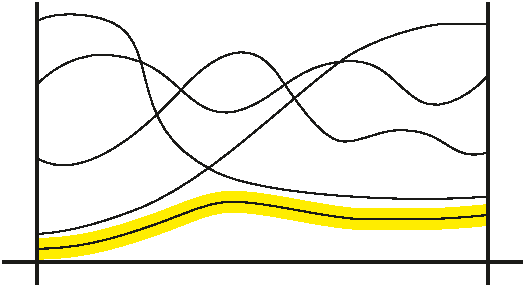
\includegraphics[width=7.5cm]{pictures/picture_3_2.pdf}};
		\draw [color=black](3.4,2.0) node[anchor=north west] {$ \RF (\theta, \delta_1 )
			$};
		\draw [color=black](3.4,1.3) node[anchor=north west] {$ \RF (\theta, \delta_2 )
			$};
		\draw [color=black](3.4,0.2) node[anchor=north west] {$ \RF (\theta, \delta_3 )
		$};
	\draw [color=black](3.4,-0.4) node[anchor=north west] {$ \RF (\theta, \delta_4 )
	$};
\draw [color=black](3.4,-.8) node[anchor=north west] {$ \RF (\theta, \delta_5 )
$};
\draw [color=black](-0.3,-1.7) node[anchor=north west] {$\Theta$};
		\end{tikzpicture}
		\caption{HPD Region (Highest Posterior Density). Pokud by nějaká funkce $ \RF (\theta, \delta_6 )
			$ náhodou na nějakém intervalu byla menší, než $ \RF (\theta, \delta_5 )
			$, tak bychom ji jednoduše zahodili.}\label{HPD}
	\end{figure}
	
	Ne vždy lze najít stejnoměrně nejlepší řešení. V~takovém případě pak přejdeme na~prostor $\Dd'_0\subset\Dd' $, kde již lze najít stejnoměrně nejlepší řešení (typicky vypustíme některé rizikové funkce), viz \ref{HPD}. Můžeme tedy optimalizovat na různých prostorech rozhodovacích funkcí, např.
	\begin{enumerate}[a)]
		\item  Prostor rozhodovacích funkcí, které jsou nestranné -- pak vede na~UMVUE.
		\item $\Dd _0$ takový, který je prostorem ekvivariantních rozhodovacích funkcí na modelech invariantních na~určitou transformaci (např. posunutí, přeškálování, tzn. tzv. \textbf{lokálně-měřítkové modely}).
	\end{enumerate}
	
	Problémy této stejnoměrně optimální strategie: \begin{enumerate}[a)]
		\item $\delta_1,\delta_2$ a~k~nim $\RF(\t,\delta_1),\RF(\t,\delta_2)$ takové, že se~kříží -- nejsme schopni rozhodnout, která strategie je lepší.
		\item Minimalizujeme $\E L$, ale $\delta$ nezávisí na~$\textbf{x}$, tedy výběr nejlepšího $\delta$ nezávisí na~naměřených datech.
		\item Na~rozmyšlenou je příklad \ref{example:problemy}.
	\end{enumerate}

\begin{example} \label{example:problemy}
	Mějme $X=\begin{cases}
	\t-1, & \PP= \frac{1}{2}, \\ \t+1, & \PP=\frac{1}{2},
	\end{cases}~\t\in\R,~\Dd =\R$. Volme
	$ L(\t,d)=1-I_\t(d)$, kde $I_\t(d)$ je 1, pokud $d=\t$ a nula, pokud ne (nazýváme ji "0-1" ztrátovou funkci).
	
	\begin{enumerate}[1)]
		\item Máme $\textbf{x}=(x_1,x_2)$ data a~sestrojíme $\delta_0(\textbf{x})=\frac{x_1+x_2}{2}=\begin{cases}
		\t\\\t-1\\\t+1
		\end{cases}$ symetricky kolem~$\t$. Potom
		$$ \RF(\t,\delta_0)=\E L(\t,\delta_0(\textbf{X}))=1-\E I_\t\big(\delta_0(\textbf{X})\big)=1-\PP\big(\delta_0(\textbf{X})=\t\big)=1-\PP(X_1\neq X_2)=\frac{1}{2}.$$ To nám říká, že střední ztráta je rovna $\frac{1}{2}$, tzn. že v~průměru 50\% případů bude příznivých (trefíme se~do~parametru).
		\item Máme data $\textbf{x}=(x_1,x_2)$ a~sestrojíme $\delta_1(\textbf{x})=x_1+1=\begin{cases}
		\t\\\t+2
		\end{cases}$ nesymetricky rozdělené kolem~$\t$. Potom
		$$\RF(\t,\delta_1)=...=1-\PP\big(\delta_1(\textbf{X})=\t\big)=1-\PP(X_1=\t-1)=\frac{1}{2}.$$
	\end{enumerate}
	Srovnání $\delta_0$ a~$\delta_1$ nelze rozhodnout na~základě $\RF$-strategie. 
\end{example}
\section{Metoda C) Strategie MINIMAXní}
\begin{define}
	 Mějme $\delta\in\Dd'$. Potom definujeme $\RF_{\sup}(\t,\delta):=\sup\limits_{\t\in\Theta} \RF(\t,\delta) \in\R^+$ jako ''\textit{maxní}''(\textit{supremální}) rizikovou funkci. Definujeme dále
	$$ \delta_0=\argmin\limits_{\delta\in\Dd'}\RF_{\sup}(\t,\delta)=\argmin\limits_{\delta\in\Dd' }\sup\limits_{\t\in\Theta}\underbrace{\E_\t L\big(\t,\delta(\X)\big)}_{\RF(\t,\delta)}.$$
\end{define}

\begin{define}
	Definujeme \textbf{minimaxní riziko} jako $\overline{\RF}=\inf\limits_{\delta\in\Dd'}\sup\limits_{\t\in\Theta}\RF(\t,\delta)$.
\end{define}

\begin{remark}
	Analogie z~teorie her. Máme 2 hráče, kteří mají antagonický vztah (snaží se~navzájem poškodit a~nezáleží jim na~ztrátě). První hráč udělá nějaký tah. Druhý hráč pak udělá tah, který co nejvíc poškodí 1. hráče. První hráč to předvídá a~snaží se~tedy minimalizovat nejhorší možnou ztrátu.
\end{remark}

\begin{figure}[h]
\centering
\begin{tikzpicture}
\node[inner sep=0pt] (pic) at (0,0)
{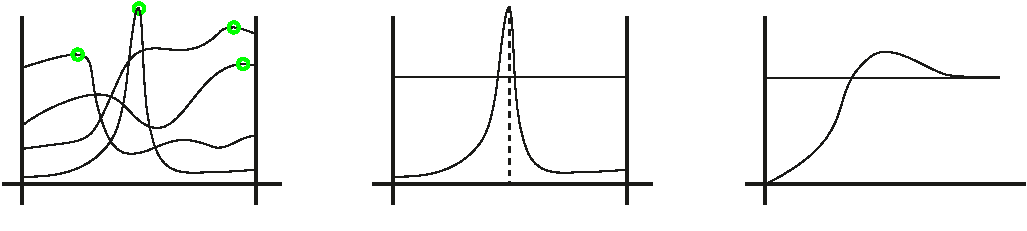
\includegraphics[width=15.0cm]{pictures/picture_3_4.pdf}};
\draw [color=black](4.2,1.5) node[anchor=north west] {$ \RF(\t,\delta_2) $};
\draw [color=black](4.7,0.1) node[anchor=north west] {$ \RF(\t,\delta_1) $};
\draw [color=black](1.6,0.9) node[anchor=north west] {$ \RF(\t,\delta_1) $};
\draw [color=black](1.6,-.4) node[anchor=north west] {$ \RF(\t,\delta_2) $};
\draw [color=black](-3.8,1.5) node[anchor=north west] {$ \RF(\t,\delta_1) $};
\draw [color=black](-3.8,1) node[anchor=north west] {$ \RF(\t,\delta_2) $};
\draw [color=black](-3.8,0) node[anchor=north west] {$ \RF(\t,\delta_3) $};
\draw [color=black](-3.8,-.5) node[anchor=north west] {$ \RF(\t,\delta_4) $};
\draw [color=black](-5.8,-1) node[anchor=north west] {$ \Theta $};
\draw [color=black](-.4,-1) node[anchor=north west] {$ \Theta $};
\draw [color=black](3.2,-1) node[anchor=north west] {$ 0 $};
\draw [color=black](4.3,-1) node[anchor=north west] {$ \left\|\Theta\right\|,~\mathrm{dim}\Theta\geq 3 $};
\end{tikzpicture}
\caption{1: zeleně suprema, nejmenší supremum je pro $\delta_2$, 2: lepší je $\delta_2$, protože ač je riziko vysoké, jeho šance je velice malá - toto je nevýhoda minimaxní strategie 3: $\delta_2$ jen lehce překmitne $\delta_1$ a~pak se~k~němu blíží asymptoticky}
\end{figure}

\section{Metoda D) Bayesovská riziková funkce} 
\begin{define}
	Nechť $\Pi=\{ \pi\}$ je množina všech apriorních rozdělení pro parametr $\t$. Definujeme \textbf{Bayesovskou rizikovou funkci} $r:\Pi\times\Dd' \to\R_0^+$ vztahem
	$$ r(\pi,\delta):=\E^\pi\big[ \RF(\t,\delta) \big]=\int\limits_{\Theta}\RF(\t,\delta)\pi(\t)\d\t=\int\limits_{\Theta}\Big( \int\limits_{\chi}L\big(\t,\delta(\textbf{X})\big)f_\textbf{X}(\textbf{x}|\t)\d\textbf{x} \Big)\pi(\t)\d\t.$$
	Definujeme dále \textbf{Bayesovskou rozhodovací funkci}, za~předpokladu existence, jako $$\delta^\pi:=\argmin\limits_{\delta\in\Dd '}r(\pi,\delta).$$ 
	Číslo $r(\pi):=r(\pi,\delta^\pi)$ nazýváme \textbf{Bayesovské (apriorní) riziko}.  

\end{define}
\begin{remark}
	Mějme $\pi$ fixní. Pak $\delta_1\leq\delta_2$ právě tehdy, když $r(\pi,\delta_1)\leq r(\pi,\delta_2)$ jsou uspořádané v~$\R^1$. To lze rozšířit i~na~nevlastní apriorní hustoty (informace), ale pouze pokud $r(\pi)<+\infty$.
\end{remark}
\begin{example}
	Mějme $X\sim\underbrace{\NN(\t,1)}_{f_X(x|\t)}$, $\t\in\R,~\pi(\t)=1$ (konstantní) na~$\R$ (nevlastní hustota, tedy nepreferujeme dopředu žádnou hodnotu). Pak
	$$ \pi(\t|x)=\frac{f_X(x|\t) \pi(\t)}{\int_{-\infty}^{+\infty}f_X(x|\t) \pi(\t)\d\t}=\frac{1}{c}\e{-\frac{1}{2}(\t-x)^2}=\frac{1}{\sqrt{2\pi}}\e{-\frac{1}{2}(\t-x)^2}=\NN(x,1).$$
	\[\begin{split}
	\delta^\pi(x)&=\EE{\pi(\t|x)}=\E\NN(x,1)=x,\\
	r(\pi)&= r(\pi,\delta^\pi)=\E^\pi \RF(\t,\delta^\pi)=\E^\pi\big[\E^f L_2\big(\t,\delta^\pi(X)\big)\big]\equal{def}\E^\pi\big[ \E^f\big(\t-\delta^\pi(X) \big)^2 \big]=\E^\pi\E^f(\t-X)^2=\\&=\E^\pi\big[ \E^f(X-\E^fX)^2 \big]=\E^\pi(\sigma^2)=\int_{-\infty}^{+\infty}\sigma^2\cdot \underbrace{\pi(\t)}_{1}\d\t=+\infty.
	\end{split}
	\]
\end{example}
\begin{define}
	Máme $L,~f_{\X},~\pi(\t)$. Definujeme \textbf{aposteriorní Bayesovskou rizikovou funkci} vztahem
	$$ \rho(\pi,\delta|\textbf{x}):=\E^\pi\big[ L\big(\t,\delta(\textbf{x})\big)|\X=\textbf{x} \big]=\int_\Theta L\big(\t,\delta(\textbf{x})\big)\pi(\t|\textbf{x})\d\t.$$ 
\end{define}

\section{Metoda E) nic nového} 
Definujeme $\delta_\rho^\pi(\textbf{x}):=\argmin\limits_{\delta}\rho(\pi,\delta|\textbf{x})$ za~předpokladu existence pro~skoro všechna $\textbf{x}$.

\begin{remark}
	Výhoda této definice je, že $\delta_\rho^\pi$ závisí přímo na~datech $\textbf{x}$. Nevýhoda pak je, že musíme minimalizaci dělat opakovaně pro~každá data $\textbf{x}$.
\end{remark}
\begin{theorem}\label{veta_zamena}
	Máme-li $\delta_\rho^\pi$ pro s.v. $\textbf{x}$, pak $\delta_\rho^\pi=\delta^\pi$, tj. je rovna s.v. Bayesovské rizikové funkci $\delta^\pi=\argmin\limits_\delta r(\pi,\delta)$ podle D strategie.
	\begin{proof}
		\[
		\begin{split}
		\rho\big(\pi,\delta_\rho^\pi(\textbf{x})|\textbf{x}\big)&\leq \rho(\pi,\delta(\textbf{x})|\textbf{x}) \hspace{0.2cm} \text{pro s.v., což víme z definice. Potom ale } \textbf{x} \\
		\E^m\rho\big(\pi,\delta_\rho^\pi(\textbf{x})|\textbf{x}\big)&\leq \E^m\rho(\pi,\delta(\textbf{x})|\textbf{x})\text{, kde } m(\textbf{x})=\int_{\Theta}f(\textbf{x}|\t)\cdot \pi(\t)\d\t.
		\end{split}
		\]
		Nyní rozepíšeme pravou stranu (potom to uděláme i s levou)
		\[
		\begin{split}
		\E^m\rho(\pi,\delta(\textbf{x})|\textbf{x})&=\int\limits_{\chi}\Big( \int\limits_{\Theta} L(\t,\delta)\underbrace{\pi(\t|\textbf{x})}_{\frac{f\pi(\t)}{\int f\pi(\t)\d\t}=\frac{f\pi(\t)}{m(\textbf{x})}}\d\t\Big)m(\textbf{x})\d\textbf{x}\equal{Fubini}\int\limits_{\Theta}\Big( \underbrace{\int\limits_{\chi} L\big(\t,\delta(\textbf{x})\big)f(\textbf{x}|\t)\d\textbf{x}}_{\E^f L=\RF(\t,\delta)} \Big)\pi(\t)\d\t=\\&=\E^\pi\E^f L=r(\pi,\delta). \\
		\E^m\rho(\pi,\delta_\rho^\pi(\textbf{x})|\textbf{x})&=\{\text{Analogický postup}\}=r(\pi,\delta_\rho^\pi).
		\end{split}
		\]
		A tedy 
		$$ r(\pi,\delta_\rho^\pi)\leq r(\pi,\delta),~\forall\delta\quad \Rightarrow\quad \delta_\rho^\pi=\delta^\pi.$$
		Závěr: D strategie Bayes ($\delta^\pi$) je rovna E strategii Bayes ($\delta_\rho^\pi(\textbf{x})$ pro s.v. $\textbf{x}$).
	\end{proof} 
\end{theorem}
Rozšíření: Máme-li $\delta_\rho^\pi(\textbf{x})$ pro s.v. $\textbf{x}$ a~stane se, že $r(\pi)=+\infty$, pak toto řešení $\delta^{\pi}$ nazveme \textbf{Zobecněnou Bayesovskou rozhodovací funkcí}.

\section{Postup při aplikaci Bayesovské strategie} 
	Můžeme postupně iterovat přes nová data. Na začátku máme znalosti o parametru $\t$ z minulosti v podobě $\pi(\t)$ a~nově naměříme data $\textbf{X}\sim f(\textbf{x}|\t)$. Za pomocí úplného Bayesovského modelu můžeme updatovat naše znalosti, přičemž získáme $\pi(\t|\textbf{x})$. Z toho můžeme například odhadnout $\widehat{\t}_\mathrm{B}$, případně interval spolehlivosti apod. Poté nová data označíme za aktuální (aposteriorní hustotu přeznačíme na apriorní) a pokračujeme dále, tedy $\widetilde{\pi}(\t)=\pi(\t|\textbf{x})$. Následně získáme nová data $\widetilde{\textbf{X}}\sim\widetilde{f}(\widetilde{\textbf{x}}|\t)$ a získáme $\widetilde{\pi}(\t|\widetilde{\textbf{x}})$... 

\section{Úloha predikce}
Zkusme porovnat klasickou a bayesovskou statistiku v úloze predikce.
\begin{description}
	\item[Klasická statistika] Předpokládáme $X\sim f(x,\t)$, aniž bychom měli apriorní informaci, a naměříme data $\textbf{x}=(x_1,...,x_n)$ jako realizaci $\textbf{X}=(X_1,...,X_n)$. Hledáme predikci (realizaci) $X_{n+1}$. Pokud jsou $X_1,...,X_n ~iid$, pak $X_{n+1}\sim f(x,\t)$ a stačí nám najít příslušné rozdělení. Proto zkusíme najít odhad závislý na $\textbf{x}$ ve tvaru $\widehat{\t}=\widehat{\t}(\textbf{x})=\widehat{\t}_{\mathrm{ML}}$. Z~toho pak získáme $\widehat{f}(x)=f(x,\widehat{\t}_\mathrm{ML})$ a~z~toho $X_{n+1}\sim\widehat{f}(x)$.
	\item[Bayesovská statistika] Opět máme $X\sim f(x|\t)$, data $\textbf{x}$ a~navíc apriorní informaci $\pi(\t)$. Máme několik možností jak pokračovat.
	\begin{enumerate}[a)]
		\item  Z~toho vypočítáme $\pi(\t|\textbf{x})$ a~z~toho získáme odhad $\widehat{\t}_\mathrm{B}=\EE{\pi(\t|\textbf{x})}$. Následně určíme hustotu $\widehat{f}(x)=f(x|\widehat{\t}_\mathrm{B})$ a pokračujeme klasicky s odhadem $X_{n+1}\sim\widehat{f}$. Bayes obecně není invariantní na tranformace, takže nemůžeme říct, že jsme získali bayesovský odhad hustoty.
		
		\item Můžeme také zkusit odhadnout přímo celou hustotu $\tau(\t)=f(x|\t)$, kde za použití apriorní hustoty $\pi(\t)$ získáme $\widehat{f}_\mathrm{B}(x)=\widehat{\tau_\mathrm{B}(\t)}$. Následní můžeme predikovat $X_{n+1}$ jako $X_{n+1}\sim\widehat{f}_\mathrm{B}$.
		
		\item \begin{define} Máme ÚBM (Úplný bayesovský model) pro $\X\sim f_{\X}(\textbf{x}|\t)$, apriorní hustotu $\pi(\t)$ a aposteriorní hustotu $\pi(\t|\textbf{x})$. Pak definujeme \textbf{Bayesovskou prediktivní hustotu} $f_\mathrm{B}^{PR} $ vztahem
		$$ f_\mathrm{B}^\mathrm{PR}(t|\textbf{x})=\int\limits_{\Theta} f_X(t|\t)\pi(\t|\textbf{x})\d\t=\E^\pi[f_X(t|\t)|\textbf{x}].$$
		\end{define}
		Potom
		$ X_{n+1}\sim f_\mathrm{B}^\mathrm{PR}(x_{n+1}|\textbf{x})$, z čehož můžeme predikovat $$\PP(X_{n+1}>b)=\int\limits_\mathrm{B}^{+\infty}f_\mathrm{B}^\mathrm{PR}\d x_{n+1}.$$
		Výhodou c) je to, že obsahuje ''plnou'' (ve smyslu integrálu) informaci aposteriorní hustoty $\pi(\t|\textbf{x})$.
	\end{enumerate}
\end{description}




\chapter{Asymptotické vlastnosti aposteriorní hustoty a~bayesovských bodových odhadů.}

\begin{define}
	Mějme $P,Q\in\mathcal{P}$ a~definujeme \textbf{totální variaci} $\TV(P,Q)=\left\|P-Q\right\|_\TV=\sup\limits_{|g|\leq 1}\left| \int g(\X)\d P-\int g(\Y)\d Q \right|\equal{ASR}\left|\begin{array}{l}
	p\equal{ozn}\frac{\d P}{\d \mu}\quad P,Q\ll\mu\\ q=\frac{\d Q}{\d \mu}
	\end{array}
	\right|=\int |p-q|\d\mu=\left\|p-q\right\|_{L_1}$.
\end{define}
\begin{define}
	Mějme posloupnost měr $(P_n)_1^{+\infty}$ a limitní míru $Q$. Řekneme, že $P_n$ konverguje silně ke $Q$, značíme $P_n\stackrel{\text{s}}{\rightarrow}Q$, pokud $\TV(P_n,Q)\to0$.
\end{define}
\begin{remark}{Připomenutí slabé konvergence}
	$$ P_n\wto Q~\Leftrightarrow~\int g(\X)\d P_n\to\int g(\Y)\d Q,\qquad \forall g\in C_\mathrm{B}^{(0)}\text{ spojité a~omezené.}$$
\end{remark}

\begin{theorem}
	$P_n\stackrel{s}{\to}Q\Rightarrow P_n\wto Q$ (AN).
\end{theorem}

\begin{proof}
	 Nechť funkce $g$ je spojitá a~omezená, $|g|\leq M$, $g^\ast =\frac{g}{M}$, $|g^\ast|\leq 1$. Pak
	$$ \left| \int g(\X)\d P_n-\int g(\Y)\d Q \right|=M\left| \int g^\ast(\X)\d P_n-\int g^\ast(\Y)\d Q \right|\leq M\cdot \left\| P-Q\right\|_\TV \stackrel{\text{LDCT}}{\longrightarrow} 0.$$
\end{proof}
\begin{theorem}[Scheffé theorem]
	Mějme $P_n,Q$ s~ASR$_\mu$, $p_n=\frac{\d P_n}{\d \mu}$, $q=\frac{\d Q}{\d \mu}$. Nechť dále hustota pravděpodobnosti $p_n\to q$ s.v. $\mu$. Pak $P_n\stackrel{s}{\longrightarrow}Q$. 
	\begin{proof}
		$$ \left| \int_A (p_n-q)\d\mu \right|\leq \int_A|p_n-q|\d\mu\leq \int_\R|p_n-q|\d\mu=2\int(p_n-q)^+\d\mu\to0,$$
		kde poslední rovnost platí, protože $\int(p_n-q)\d\mu=0$, a~tedy $\int(p_n-q)^+\d\mu-\int(p_n-q)^-\d\mu=0$.	\end{proof}
\end{theorem}
\begin{remark} Z~01MAS víme, že pro~$\fregmle$ platí, že \begin{enumerate}[1)]
		\item $\supp f$ nezávisí na~$\t$,
		\item $f\in\mathcal{C}^{(3)}$ vzhledem k~$\t$ pro s.v. $x\in\supp f$,
		\item $\int f_\t'=0$ a~$\int f_{\t\t}''=0$,
		\item $\left( \mathbb{J}(\t) \right)_{i,j}=\EE{\frac{\partial\log f}{\partial \t_i}\cdot\frac{\partial\log f}{\partial \t_j}}=-\EE{\frac{\partial^2 \log f}{\partial\t_i \partial \t_j}}$, $\mathbb{J}(\t)$ je PD a~konečná pro~$\forall\t\in\Theta$,
		\item $\forall\t_0~\exists H_{\t_0}~\exists M(\X)\in\LL_1(P_{\t_0})$ tak, že $\left\| \frac{\partial^3\log }{\partial \t^3}\right\|\leq M(x)$ na~$H_{\t_0}$, kde $\E_{\t_0}[M(X)]<+\infty$.
	\end{enumerate}
\end{remark}
\begin{theorem}[Bernstein - von Mises]
	Předpokládejme ÚBM. Potom $X\sim f(x|\t)$ vzhledem k míře $\lambda$, která je $\sigma$-finitní, $\mathcal{F}=\left\{ f(x|\t):\t\in\Theta\subset \R^k \right\}$, $\Theta$ otevřená, $\t\sim\pi(\t)$ vlastní hustota, spojitá a $\pi(\t)>0$ (Tedy máme $\varphi(x,\t)=f\cdot\pi$, $m(\textbf{x})=\int f\cdot \pi\d\t$, $\pi(\t|\textbf{x})=\varphi/m=\frac{f\cdot\pi}{\int f\cdot\pi\d\t}$). Nechť dále $\mathcal{F}=\fregmle$. Pak
	$$ \left\| \pi(\t|\textbf{x})-f_{\NN\left( \widehat{\t}_n,\frac{1}{n}\mathbb{J}^{-1}(\t_0) \right)} \right\|_{TV}\to0 \hspace{0.2cm}\text{ pro }\forall \t_0,$$
	kde $\widehat{\t}_n$ je konzistentní řešení $LE_Q$, tzn. $\widehat{\t}_n$ řeší $\frac{\partial \log f}{\partial \t_j}=0,~\forall j\in\hat{k}$.
\end{theorem}
\begin{dusl}
	Mějme $\fregmle$, $\pi(\t)>0$ vlastní hustota a spojitá, $\t_0$ skutečná hodnota parametru $\t$. Pak $(\t|\textbf{x})\sim\AN\big(\htn(\textbf{x}),\frac{1}{n}\mathbb{J}^{-1}(\t_0)\big)$ pro~$\forall\t_0$.
	
	Závěr: $\sqrt{n}\big( (\t|\textbf{x})-\htn(\textbf{x}) \big)\Dto \NN\big( 0,\mathbb{J}^{-1}(\t_0) \big),~\forall\t_0$. Bayesovská strategie je asymptoticky ekvivalentní MLE.
	\begin{proof}
		$k=1$: Máme $f_{X},~(X_j)_1^n,~f_{X_j}(x_j|\t),~f_n\equal{id}\prod_1^n f_{X_j}=f_n(\textbf{x}|\t),~\pi(\t|\textbf{x})=\frac{f_n \pi}{\int f_n \pi\d\t}$. Transformujeme pomocí $g: t=\sqrt{n}\big( \t|\textbf{x}-\htn \big)$, kde $\htn$ je ELE (konzistentní řešení $LE_Q$), $g^{-1}:\t|\textbf{x}=\htn + \frac{t}{\sqrt{n}}$, $\mathbb{J}_{g^{-1}}=\frac{1}{\sqrt{n}}>0$. Potom transformujeme
		\[
		\begin{split}
		\t|\textbf{x}&\sim\pi(\t|\textbf{x}),\\
		\sqrt{n}\big(\t|\textbf{x}-\htn\big)&\sim\frac{f_n\big(\textbf{x}|\htn+\frac{t}{\sqrt{n}}\big)\pi\big( \htn+\frac{t}{\sqrt{n}} \big)\big(\frac{1}{\sqrt{n}}\big)}{\int f_n(\textbf{x}|\t)\pi(\t)\d\t}=\left|\begin{array}{l}
		\t=\htn+\frac{s}{\sqrt{n}}\\\d\t=\frac{\d s}{\sqrt{n}}\end{array}
		\right|=\\ &=\frac{f_n\big(\textbf{x}|\htn+\frac{t}{\sqrt{n}}\big)\pi\big( \htn+\frac{t}{\sqrt{n}} \big)}{\int f_n\big(\textbf{x}|\htn+\frac{s}{\sqrt{n}}\big)\pi\big( \htn+\frac{s}{\sqrt{n}} \big)\d s}.
		\end{split}
		\]
		Máme spojité $\partial_\t^3$, a~proto rozvineme pomocí Taylora $\log f_n$ do~2. řádu:
		\[
		\begin{split}
		\log f_n(\textbf{x}|\htn+\frac{t}{\sqrt{n}})&=\log f_n(\textbf{x}|\htn)+0\text{\footnotemark}+\frac{1}{2}\frac{t^2}{n}\frac{\partial^2 \log f_n}{\partial\t^2}\Big|_{\t=\htn}+R_n=\\&=\log f_n(\textbf{x}|\htn)+\frac{t^2}{2}\underbrace{\Big( \frac{1}{n}\sumjn \frac{\partial^2 \log f_{X_j}(x_j|\htn)}{\partial\t^2} \Big)}_{\xrightarrow[\text{ZVČ}]{\PP_{\t_0}}\EE{\frac{\partial^2\log f_X}{\partial\t^2}}=-\mathbb{J}(\htn)\wedge \htn \stackrel{\PP_{\t_0}}{\rightarrow} \t_0}+\underbrace{R_n}_{\xrightarrow[(s.j.)]{\PP_{\t_0}}0}.
		\end{split}
		\]
		\footnotetext{$\frac{\partial \log f_n}{\partial \t}|_{\t=\htn}=0$, protože $\htn$ je řešením soustavy věrohodnostních rovnic}
		Z toho potom plyne, že $f_n\big(\textbf{x}|\htn+\frac{t}{\sqrt{n}}\big)=f_n(\textbf{x}|\htn)\e{-\frac{t^2}{2}\mathbb{J}(\htn)}\cdot\widetilde{R}_n$ a~tedy \[
		\begin{split}
		\pi(t|\textbf{x})&=\frac{f_n\e{-\frac{t^2}{2}\mathbb{J}(\htn)}\cdot\widetilde{R}_n \pi\big( \htn+\frac{t}{\sqrt{n}} \big)}{f_n\int \e{-\frac{s^2}{2}\mathbb{J}(\htn)}\widetilde{R}_n \pi\big(\htn+\frac{s}{\sqrt{n}}\big)\d s}\xrightarrow[(n\rightarrow \infty)]{\PP_{\t_0}\text{\footnotemark}}\frac{\e{-\frac{t^2}{2}\mathbb{J}(\t_0)}\cdot1\cdot \pi(\t_0)}{\int\e{-\frac{s^2}{2}\mathbb{J}(\t_0)}\cdot1\cdot\pi(\t_0)\d s}=\left| \begin{array}{l}
		u=s\sqrt{\mathbb{J}(\t_0)}\\\d s=\frac{\d u}{\sqrt{\mathbb{J}(\t_0)}}		
		\end{array}
		\right|=\\&=\frac{\sqrt{\mathbb{J}(\t_0)}}{\sqrt{2\pi}}\e{-\frac{t^2}{2}\mathbb{J}(\t_0)}\sim\NN\Big( 0,\frac{1}{\mathbb{J}(\t_0)} \Big).
		\end{split}
		\]
		\footnotetext{Záměna limity a integrálu: z MIPu známe větu, která říká, že v případě hustot a integrací dle pravděpodobnostní míry, že nepotřebujeme Lebesgueovskou majorantu}
	\end{proof}
\end{dusl}
\begin{theorem}
	Mějme ÚBM, $f_X$, $\pi(\t)>0$ omezenou a~vlastní. Označme $\pi(\t|\textbf{x})=\frac{f\cdot\pi}{\int f\cdot\pi\d\t},~\pi_0(\t|\textbf{x})=\frac{f\cdot1}{\int f\cdot1 \d\t}$, kde $\int f\cdot\pi\d\t<+\infty$ a~$\int f\cdot1 \d\t<+\infty$. Pak
	$$ \left\|\pi(\t|\textbf{x})-\pi_0(\t|\textbf{x})\right\|_\TV\leq \max\Big(\frac{a+b}{1-a},\frac{a+b+ac}{1+a+b+ac}\Big)+\frac{a(2-a+c)}{1-a}=\epsilon_{a,b,c},$$
	kde $a\in\langle 0,1),~b>0,~c>0$, jsou definovány následovně:\begin{enumerate}[1)]
		\item $\exists A\subset \Theta$ tak, že $\int_A \pi_0(\t|\textbf{x})\d\t\geq 1-a$,
		\item $\inf_A \pi(\t)=m>0$,
		\item $\sup_A \pi(\t)\leq (1+b)m$,
		\item $\sup\limits_{\Theta\setminus A} \pi(\t)\leq(1+c)m$. 
	\end{enumerate}
\end{theorem}
\begin{proof}
Bez důkazu.
\end{proof}
\begin{dusl}
	Pokud dokážeme stlačit horní hranici $\epsilon_{a,b,c}$ k~nule, tak v~$\TV$ jsou $\pi(\t|\textbf{x})$ a~$\pi_0(\t|\textbf{x})$ velmi blízko. Potom tedy $\widehat{\t}_\mathrm{B}^\pi=\EE{\pi(\t|\textbf{x})}$ a~$\widehat{\t}_\mathrm{B}^1=\EE{\pi_0(\t|\textbf{x})}$ jsou blízko. To znamená, že vliv $\pi(\t)$ se~ztrácí.
\end{dusl}
\begin{remark}
	$\epsilon_{a,b,c}$ chceme malé. Potřebujeme $a,b$ malé, $c$ ne příliš velké.
\end{remark}
	
%\begin{figure}[h]
%	\centering
%	\begin{tikzpicture}
%	\node[inner sep=0pt] (pic) at (0,0)
%	{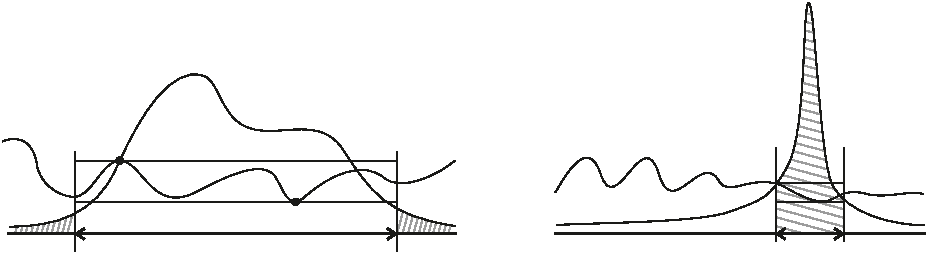
\includegraphics[width=15.0cm]{pictures/picture_4_1.pdf}};
%	\draw [color=black](3,0.5) node[anchor=north west] {$ \delta $};
%	\draw [color=black](0,-0.3) node[anchor=north west] {$ \theta $};
%	\end{tikzpicture}
%	\caption{popis}
%\end{figure}
	



\chapter{Princip neurčitosti}

Problém principu neurčitosti spočívá v tom, že máme možnost volit nevlastní apriorní hustotu ve tvaru $\pi(\t)=c$ na~$\Theta$, což znamená, že původně o parametru $\t$ vůbec nic nevíme. Z fyzikální podstaty můžeme třeba vědět jen to, že se parametr nachází na $\R^+$. Uveďme příklad tohoto problému.
\begin{example}
	Mějme ÚBM, $X\sim f(x|\t),~\t\in(0,1),~\pi(\t)=1$ na~$(0,1)$. Podle Bayese získáme aposteriorní hustotu $\pi(\t|\textbf{x})$ a z ní můžeme provést odhad $\widehat{\t}_\mathrm{B}(\textbf{x})$. Představme si nyní, že budeme chtít místo parametru odhadnout např. odmocninu z tohoto parametru. Označme tedy $\eta=\t^2$, $\t=\sqrt{\eta}$. Po dosazení do původní hustoty získáme reparametrizaci $$f(x~|~\t=\sqrt{\eta})=f(x|\eta).$$ $\t$ považujeme za~znáhodněné (apriorně předpokládáme, že o~$\t$ nic nevíme). Transformace hustoty, $\t$ na~$\eta$ probíhá jako $$\pi_H(\eta)=\pi(\underbrace{\sqrt{\eta}}_{\t})\cdot\big|\mathbb{J}_H(\eta)\big|=1\cdot\frac{1}{2\sqrt{\eta}}=\frac{1}{2\sqrt{\eta}},$$
	kde $\pi_H$ značíme obecně transformovanou informaci. Je paradoxní, že o~$\t$ nemáme konkrétní apriorní informaci a~přitom o~$\eta=\t^2$ víme, že je nevlastní (viz obr. \ref{fig:p71}).
\begin{figure}[h]
	\centering
	\begin{tikzpicture}
	\node[inner sep=0pt] (pic) at (0,0)
	{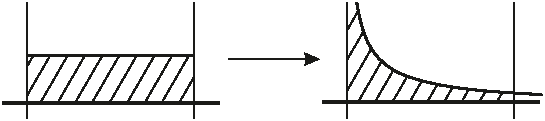
\includegraphics[width=12.0cm]{pictures/picture_4_2.pdf}};
	\draw [color=black](3,0.23) node[anchor=north west] {$ \pi_H(\eta) $};
 	\draw [color=black](-4,0.73) node[anchor=north west] {$ \pi(\theta) $};
 	\draw [color=black](-1.3,0.8) node[anchor=north west] {transformace};
 	\draw [color=black](-5.87,-0.95) node[anchor=north west] {$ 0 $};
 	\draw [color=black](-1.65,-0.95) node[anchor=north west] {$ 1 $};
 	\draw [color=black](1.13,-0.95) node[anchor=north west] {$ 0 $};
 	\draw [color=black](5.4,-0.95) node[anchor=north west] {$ 1 $};
	\end{tikzpicture}
	\caption{Znázornění transformace $\pi(\t)$. O $\t$ nemáme konkrétní apriorní informaci, ale o $\eta=\t^2$ víme, že je nevlastní (není ani integrovatelná na 1). To ukazuje problém principu neurčitosti.}
	\label{fig:p71}
\end{figure}

\end{example}
\section{Jeffreysova hustota}
	Mějme $X\sim f(x|\t),~\t\in\Theta,~\t\sim\pi(\t),~\mathcal{F}=\{f(x|\t)\}$. Zavedeme reparametrizaci $\eta=\inv{H}(\t)$, tzn. $\t=H(\eta)$. 
	$$ f_H(x|\eta)=f\big(x|\t=H(\eta)\big)=f\big(x|H(\eta)\big),\quad\text{takto získáme }\mathcal{F}_H.$$
	Z $\pi(\t)$ vytvoříme $\pi_H(\eta)=\pi\big(H(\eta)\big)\cdot\big|\mathbb{J}_H(\eta)\big|$, kde  $\mathbb{J}_H(\eta)$ je Jacobián.
	Z ÚBM $\{\mathcal{F},\pi\}$ potom plyne aposteriorní hustota $\pi(\t|\textbf{x})~\to~\widehat{\t}_\mathrm{B}(\textbf{x})=\EE{\pi(\t|\textbf{x})}$. Dále z~ÚBM $\{\mathcal{F},\pi\}$ plyne ÚBM $\{\mathcal{F}_H,\pi_H\}$ a~z~něho aposteriorní hustota $\pi(\eta|\textbf{x})$ a následně $ \widehat{\eta}_\mathrm{B}(\textbf{x})=\EE{\pi(\eta|\textbf{x})}$. 
	
	Pozor na~$\widehat{\t}_\mathrm{B}\neq H(\widehat{\eta}_\mathrm{B})$! To může být problém.
	
\begin{theorem}[Jeffreys]
	Máme ÚBM $\mathcal{F},\pi(\t),~\eta=\inv{H}(\t),~\t=H(\eta)$ a~předpokládejme, že $\t\in\Theta\subset\R^k$ a~že $H$ je regulární transformace. Nechť $\mathcal{F}$ je regulární systém hustot ($\fregp$). Po reparametrizaci máme $\mathcal{F}_H$ a $\pi_H$. Volme $\pi(\t)=\sqrt{\det \mathbb{I}(\t)}$, kde $\mathbb{I}(\t)$ je Fishera informační matice pro~$\t$ v~$\mathcal{F}$. Pak $\pi_H(\eta)=\sqrt{\det \mathbb{I}_H(\eta)}$ v $\mathcal{F}_H$ a~platí, že 
	$$ \int_\mathrm{B}\pi(\t|\textbf{x})\d\t=\int_{\inv{H}(B)}\pi_H(\eta|\textbf{x})\d\eta,\qquad\forall B\in\Bb_\Theta \text{ (B je borelovská množina).}$$
	\begin{proof}
		Pro $k=1$: (zbytek ponechán čtenáři ;) ) Nejprve tedy spočítáme
		\[
			\begin{split}
			\int_\mathrm{B}\pi(\t|\textbf{x})\d\t&=\frac{1}{c}\int_\mathrm{B} f(\textbf{x}|\t)\pi(\t)\d\t=\left|\begin{array}{c}
			\t=H(\eta)\\\mathbb{J}_H(\eta)
			\end{array}
			\right|=\frac{1}{c}\int_{\inv{H}(B)}\underbrace{f\big(\textbf{x}|H(\eta)\big)}_{f_H(\textbf{x}|\eta)}\underbrace{\pi\big(H(\eta)\big)\cdot\big|\mathbb{J}_H(\eta)\big|}_{\pi_H(\eta)}\d\eta=\\&=\frac{1}{c}\int_{\inv{H}(B)}f_H(\textbf{x}|\eta)\pi_H(\eta)\d\eta=\int_{\inv{H}(B)}\pi(\eta|\textbf{x})\d\eta,
			\end{split}
			\]
		neboť $c$ je v obou případech stejné. Protože platí, že
			$$ \mathbb{I}_H(\eta)=\EE{\frac{\partial\log f_H(\eta)}{\partial\eta}}^2=\EE{\frac{\partial\log f(x|H(\eta))}{\partial\t}\frac{\partial H(\eta)}{\partial\eta}}^2=\mathbb{I}\big(H(\eta)\big) \cdot \mathbb{J}_H^2(\eta) ,$$
			pak \[
			\begin{split}
			\pi_H(\eta)&=\pi\big(H(\eta)\big)\cdot\big|\mathbb{J}_H(\eta)\big|=\sqrt{\det \mathbb{I}\big(H(\eta)\big)}\cdot\big|\mathbb{J}_H(\eta)\big|=\sqrt{\det \mathbb{I}_H(\eta)\mathbb{J}_H^{-2}(\eta)}\cdot\big|\mathbb{J}_H(\eta)\big|=\\&=\sqrt{\det \mathbb{I}_H(\eta)}.
			\end{split}
			\]
			Získali jsme tedy $\pi(\t)=\sqrt{\det \mathbb{I}(\t)}$, což je \textbf{Jeffraysova apriorní hustota} (nebo také Jeffreysův princip neurčitosti).
	\end{proof}
\end{theorem}
Tedy pokud obecně o parametru $\t$ nevíme nic, tak máme 2 možnosti. Můžeme na celém oboru zvolit $\pi(\t)=1$, ale nebudeme mít zaručenou invarianci na reparametrizaci. Druhou možností je právě zvolit Jeffreysovu apriorní hustotu, která často není vlastní, ale můžeme pak použít Jeffreysovu větu. Pojďme si to ukázat na nějakém příkladu.
\begin{example}
	Mějme $X\sim f_X(x|\lambda)=\mathrm{Po}(\lambda)$, tzn. $f_{X_j}=\frac{\lambda^{x_j}}{x_j!}\e{-\lambda},~f_\textbf{X}(\textbf{x}|\lambda)=\frac{\lambda^{\sum x_j}}{\prod x_j!}\e{-n\lambda},~\lambda~>~0$.\begin{enumerate}[a)]
		\item Pokud je $\lambda$ neznámé, pak $\pi(\lambda)=1$ na~$\R^+$ (nevlastní). (Je jedno, jestli vezmeme rovno 1 nebo nějaké jiné konstantě.)
		$$
		\pi(\lambda|\textbf{x})=\frac{\fex \pi}{\underbrace{\int_{0}^{+\infty}\fex\pi\d\lambda}_{<+\infty}}=\underbrace{\frac{1}{c}\frac{1}{\prod x_j!}}_{\frac{1}{c'}}\lambda^{\sumjn x_j}\e{-n\lambda}\sim\mathrm{Gamma}\Big(\sumjn x_j+1,n\Big).$$
		
		Pro připomenutí: $\frac{1}{c'}x^{\alpha-1}e^{-\beta x}=\frac{\beta^{\alpha}}{\Gamma(\alpha)}x^{\alpha-1}e^{-\beta x } \sim \mathrm{Gamma}(\alpha,\beta) $
		
		Bayesovský odhad pak bude ve tvaru
		 $$\widehat{\lambda}_\mathrm{B}=\E\Big[\mathrm{Gamma}\Big(\underbrace{\sum x_j+1}_{\alpha},\underbrace{n}_\beta\Big)\Big]=\frac{\alpha}{\beta}=\frac{1}{n}\sumjn x_j+\frac{1}{n}=\Oxn+\frac{1}{n}\sim \Oxn~(\text{MLE pro velká }n).$$
		\item Jeffreys: Zkonstuujeme apriorní informaci jako $$\pi(\lambda)=\sqrt{\det \mathbb{I}(\lambda)}=\sqrt{\det \EE{-\frac{\partial^2\log\fex}{\partial\lambda^2}}}=\sqrt{n\cdot\frac{1}{\lambda}}=\sqrt{n}\frac{1}{\sqrt{\lambda}}.$$
		Volíme $\pi(\lambda)=\frac{1}{\sqrt{\lambda}}$. V apriorní informaci nehraje konstanta roli, protože se vždy v Bayesově vzorci pokrátí, tedy můžeme vypustit $\sqrt{n}$.
		$$ \pi(\lambda|\textbf{x})=\frac{f(\textbf{x}|\lambda) \pi(\lambda)}{\underbrace{\int f(\textbf{x}|\lambda)\pi(\lambda)\d\lambda}_{<+\infty}}=\frac{1}{c'}\lambda^{\sum_{j=1}^n x_j-\frac{1}{2}}\e{-n\lambda}\sim\mathrm{Gamma}\Big(\underbrace{\sumjn x_j+\frac{1}{2}}_{\widetilde{\alpha}},\underbrace{n}_{\widetilde{\beta}}\Big).$$
		Bayesovský odhad $\widehat{\lambda}_\mathrm{B}^J=\EE{\mathrm{Gamma}(\widetilde{\alpha},\widetilde{\beta})}=\frac{\widetilde{\alpha}}{\widetilde{\beta}}=\Oxn+\frac{1}{2n}\sim\Oxn$ (MLE pro velká $n$).
	\end{enumerate}
	Pro malá $n$ se odhady v a) a b) liší.
\end{example}

\chapter{Konjugované systémy apriorních hustot, princip maximální entropie, limitní aposteriorní hustoty, příklady.}

\section{Limitní aposteriorní hustoty ($\widehat{\t}_\mathrm{B}$)}
Mějme ÚBM $\{\mathcal{F},\pi(\t)\}$ a~předpokládejme, že $\pi\in\mathcal{H}:=\{\pi(\t,\boldsymbol{\lambda}):\boldsymbol{\lambda}\in\Lambda\}$. Volme $\lambda_0\in\partial\Lambda$ z hranice a~definujme limitní apriorní hustotu $\pi_{\lambda_0}(\t)=\lim\limits_{\substack{
		\lambda\to\lambda_0\\\lambda\in\Lambda	}
}c\cdot \pi(\t,\lambda)$, která bývá často nevlastní. 

Dále pak vyjádříme limitní aposteriorní hustotu (za předpokladu záměny integrálu a~limity v parametrickém integrálu) $$\pi_{\lambda_0}(\t|\textbf{x})\equal{ozn}\frac{f\pi_{\lambda_0}(\t)}{\int_\Theta f\pi_{\lambda_0}(\t)\d\t}=\frac{f\lim\limits_{\lambda\to\lambda_0}c\pi(\t,\lambda)}{\int_\Theta f\lim\limits_{\lambda\to\lambda_0}c\pi(\t,\lambda) \d\t}=\lim\limits_{\substack{
		\lambda\to\lambda_0\in\partial\Lambda\\\lambda\in\Lambda	}
}\frac{f\pi(\t,\lambda)}{\int f\pi(\t,\lambda)\d\t}=\lim\limits_{\lambda\to\lambda_0}\pi(\t|\textbf{x},\lambda).$$
Z toho vyplývá, že $\htb^\mathrm{lim} =\EE{\pi_{\lambda_0}(\t|\textbf{x})}$, což často vede na~nějakou~klasickou statistickou proceduru.

\begin{example}
	Mějme $X\sim f_X=\mathrm{Exp}(\t),~f_X=\theta\e{-\t x},~\t>0$, $$\mathcal{H}=\{\t\sim\mathrm{Gamma}(\alpha,\beta),~\text{tzn. }\pi\big(\t,\underbrace{(\alpha,\beta)}_{\boldsymbol{\lambda}}\big)=\t^{\alpha-1}\e{-\beta\t}\},~\Lambda=\R^{2+}.$$ $\boldsymbol{\lambda}_0=(0,0)\in\partial\Lambda\Rightarrow\pi_{0,0}(\t)=\lim\limits_{(\alpha,\beta)\to(0,0)^{+}}\t^{\alpha-1}\e{-\beta\t}=\frac{1}{\t}$ (nevlastní).
	$$\pi_{(0,0)}(\t|\textbf{x})=\frac{f\cdot\frac{1}{\t}}{\underbrace{\int_{0}^{+\infty}f\cdot\frac{1}{\t}\d\t}_{<+\infty}}\equal{iid}\frac{\t^n e^{-\t\sumjn x_j}\cdot\frac{1}{\t}}{c}=\frac{1}{c}\t^{n-1}\e{-\t\sumjn x_j}\sim\mathrm{Gamma}\Big(n,\sumjn x_j\Big),$$
	$$\htb^{\mathrm{lim}}=\E\Big[\mathrm{Gamma}\Big(n,\sumjn x_j\Big)\Big]=\frac{n}{\sumjn x_j}=\inv{(\Oxn)}=\html.$$
	Pokud bychom chtěli dostat pouze $\Oxn$, tak bychom v $\mathcal{H}$ museli namísto $\mathrm{Gamma}$ rozdělení použít inverzní $\mathrm{Gamma}$ rozdělení.
\end{example}
\begin{example}
	Volba $\pi(\t)$? Subjektivní. New England Journal of Medicine - studie\begin{enumerate}[1)]
		\item léčba rakoviny plic - operace - víme, že šance na~přežití je 68\%, ale jen 44\% lidí by tam šla. 
		\item léčba rakoviny plic - operace - víme, že pravděpodobnost úmrtí je 32\%, ale jen 18\% lidí by tam šla. 
	\end{enumerate}
\end{example}

\subsection{Empirical Bayes}
Máme $\mathcal{H}=\{\pi(\t,\lambda):\lambda\in\Lambda\}$. Spočítá se marginální rozdělení $m_\lambda(\textbf{x})=\int_\Theta\underbrace{f(\textbf{x}|\t)\pi(\t,\lambda)}_{\phi(\textbf{x},\t,\lambda)}\d\t$. Vezmete data $\textbf{X}$, realizace $\textbf{x}$ a  na~základě dat odhadneme klasickou statistickou procedurou (např. $\lambda_{\mathrm{ML}}$ - maximálně věrohodný odhad) $\widehat{\lambda}(\textbf{x})$ v $m_\lambda(\textbf{x})$ a~provedeme Bayesovský princip s~apriorní hustotou $\pi(\t,\widehat{\lambda}_{\mathrm{ML}})$ klasickou statistickou procedurou $\widehat{\lambda}_{\mathrm{ML}}$.

2. možnost volby - principem ME (maximální entropie) $H(\pi)=-\int_\Theta\pi(\t)\log \pi(\t)\d\t$. $\pi$~volíme tak, aby $H(\pi)$ bylo maximální.

%%%%%%%%%%%%%%%%%%% lesson 8

Máme tedy omezení ve formě $\E^\pi[g_i(\t)]=\omega_i,~\forall i\in K$. Maximální $H(\pi)$ vazebné je $$\pi^K(\t_i)=\frac{\e{\sumjn \lambda_j g_j(\t_i)}}{\sum \e{\sumjn \lambda_jg_j(\t_i)}},~\forall i,$$
kde $\lambda_j$ jsou Lagrangeovy koeficienty.

Pro spojitý model:

$$ KL(\pi,\pi_0)=\E^\pi\big[\log\frac{\pi_0}{\pi}\big]=\int\pi\log\frac{\pi_0}{\pi}\d\t \text{, kde KL je Kulback-Leiblerova vzdálenost}.$$
Pokud $\pi_0=1$, pak $KL(\pi,1)=-\int\pi\log\pi=H(\pi)$. Naše volba $\pi$ závisí na $\pi_0$.

\begin{define}[Konjugované systémy apriorních hustot]
	Mějme systém hustot $\mathcal{F}=\{f(x|\t):\t\in\Theta\subset\R^k\}$ a označme $\mathcal{H}$ systém apriorních hustot pro $\t$. Pak $\mathcal{H}$ nazveme \textbf{konjugovaný systém apriorních hustot} pro $\mathcal{F}$, pokud $\pi(\t|\textbf{x})\in\mathcal{H}$.
\end{define}
\begin{theorem}
	Mějme $\mathcal{F}_n=\{\fex(\textbf{x}|\t)=\prod_{j=1}^n f_{X_j}(x_j|\t)\} ~id$ a předpokládejme, že $T_n(\textbf{X})$ je postačující statistika pro $\mathcal{F}_\textbf{X}$, tzn. dle Neymannova faktorizačního kritéria $\fex(\textbf{y}|\t)=h_n(\textbf{y})g_n\big(\t,T_n(\textbf{y})\big),$ $\forall\t,\forall\textbf{y},\forall n$. Pak $$\mathcal{H}=\bigg\{\frac{g_m(\boldsymbol{\t},\textbf{t})}{\int_{\Theta} g_m(\boldsymbol{\t},\textbf{t})\d\t}:\forall m\in\N,\forall\textbf{t}\in S_m,\text{ kde }S_m=\{\textbf{t}:\exists\textbf{y},\text{ že }T_m(\textbf{y})=\textbf{t}\}\bigg\}$$
	je Conjugated Family (CF). (Konjugovaný systém apriorních hustot)
	\begin{proof}
		Volíme apriorní hustotu $\pi(\t)\in\mathcal{H}$, tzn. $\pi(\t)\sim g_m(\t,\textbf{t})$. Z toho vyplývá, že $\exists\textbf{y}$ tak, že $T_m(\textbf{y})=\textbf{t}$. Dále platí, že \[
		\begin{split}
		\pi(&\t|\underbrace{\textbf{x}}_{\dim n})\sim f_n(\textbf{x}|\t)\cdot g_m(\t,\textbf{t})\sim \underbrace{g_m\big(\t,T_m(\textbf{y})\big)\cdot h_m(\textbf{y})}_{NFK\Rightarrow f_m(\textbf{y}|\t)}\cdot f_n(\textbf{x}|\t)=f_m(\textbf{y}|\t)\cdot f_n(\textbf{x}|\t)=\\&=\prod_{j=1}^mf(y_j|\t)\prod_{j=1}^nf(x_j|\t)=\prod_{j=1}^{m+n}\underbrace{f_{Z_j}(z_j|\t)}_{\textbf{z}=(\textbf{y},\textbf{x})}=f_{m+n}(\textbf{z}|\t)\overset{\text{NFK}}{=}\underbrace{h_{n+m}(\textbf{z})}_{\text{konst}}\cdot g_{n+m}\big(\t,\underbrace{T_{n+m}(\textbf{y})}_{\textbf{t}\in S_{n+m}}\big)\sim g_{n+m}(\t,\textbf{t})
		\end{split}
		\]
		
		Z tohoto důkazu jsme dostali přirozenou CF.
		
		Vhodným rozšířit na $m\in\R$ vznikne obvyklá CF.
	\end{proof}
\end{theorem}
\begin{example}
	Mějme $X\sim f_X(x|\t)=\Exp(\lambda)$, $f_X=\lambda\e{-\lambda x},~\lambda>0$. $$\mathcal{F}_n: ~f_n(\textbf{x}|\underbrace{\t}_{\lambda})=\lambda^n\e{-\lambda\sumjn x_j}=\left|\begin{array}{c}
	ozn.~T_n(\textbf{x})=\sumjn x_j\\\text{je postač. stat. pro }\mathcal{F}_n
\end{array}
\right|=1\cdot g_n\big(\lambda,T_n(\textbf{x})\big).$$
Označme $$\sumjn x_j=t~\Rightarrow~\mathcal{H}=\Big\{ \frac{g_m(\lambda,t)}{c}:m\in\N,~t\in S_m,... \Big\}=\Big\{\underbrace{\lambda^m\frac{\e{-\lambda t}}{c}}_{\mathrm{Gamma}(m+1,t)}:m\in\N,t\in S_m=\{\textbf{t}=\sum_{j=1}^m x_j \}=\R^+\Big\},$$
čímž jsme získali přirozenou CF.

Opět lze rozšířit na obvyklou CF, tj. $\mathrm{Gamma} (\alpha,\beta)=\mathcal{H}_{obv}$, $\alpha,\beta >0$ (rozšíření v $\alpha$, $\mathbb{N}\rightarrow \R^{+}$).

Jelikož $X\sim\Exp(\lambda),~\pi(\lambda)=\mathrm{Gamma}(\alpha,\beta)$, pak 
$$ \pi(\lambda|\textbf{x})=\frac{\lambda^n\e{-\lambda\sum x_j}\frac{1}{c}\lambda^{\alpha-1}\e{-\lambda\beta}}{\int_{0}^{+\infty}\lambda^n\e{-\lambda\sum x_j}\frac{1}{c}\lambda^{\alpha-1}\e{-\lambda\beta}\d\lambda}=\frac{\lambda^{n+\alpha-1}\e{-\lambda(\sum x_j+\beta)}}{c}\sim\mathrm{Gamma}\big(n+\alpha,\sumjn x_j+\beta\big)\in\Hobv .$$

Seznam CF: \begin{enumerate}[a)]
	\item $X\sim \mathrm{Bi}(n,p)\Rightarrow CF~\mathcal{H}=\{\pi(p)\sim\mathrm{Beta}(\alpha,\beta)\}$,
	\item $X\sim\mathrm{Poisson}(\lambda)\Rightarrow CF~\mathcal{H}=\{\pi(\lambda)\sim\mathrm{Gamma}(\alpha,\beta)\}$,
	\item $X\sim U(0,\t),~\t\in\R^+\Rightarrow CF~\mathcal{H}=\{\pi(\t)\sim\mathrm{Pareto}(a,b)\}$, kde Paretovo rozdělení je mocninného typu $\t\sim\frac{a}{b}\big(\frac{b}{\t}\big)^{a+1},~\t\geq b$, které má těžké chvosty.
	\item \begin{enumerate}[1)]
		\item $X\sim \NN(\mu,\sigma_0^2),~\sigma_0>0$ a známé, pak postačující statistika je ve tvaru $T_n(\textbf{X})=\sumjn X_j\in\R$. Potom $$\mathcal{H}_{CF_{obv}}=\big\{\pi(\mu)\sim\NN(a,b^2),~a\in\R,b>0\big\}$$ a parametry $a,b$ ladíme tvar apriorní informace.
		\item $X\sim\NN(\mu_0,\sigma^2),~\mu_0$ známe. Pak postačující statistika je ve tvaru $T_n(\textbf{X})=\sumjn(X_j-\mu_0)^2$, protože 
		$$ \fex=\underbrace{\frac{1}{c}\e{-\frac{1}{2\sigma^2}\sumjn(X_j-\mu_0)^2}}_{g_n(t,\sigma^2)},$$ a proto $\Hobv$ pro parametr $\underbrace{\frac{1}{\sigma^2}}_{\t}=\{\pi(\t)\sim\mathrm{Gamma}(\alpha,\beta)\}.$
		\item $X\sim\NN(\mu,\sigma^2)$. Pak $T_n(\textbf{X})=\Big(\sumjn X_j,\sumjn X_j^2\Big)\in\R\times\R_0^+$ je postačující statistika, a proto
		$\Hobv$ pro $(\mu,\frac{1}{\sigma^2})$ definujeme tak, že $\pi\big(\mu|\frac{
		1}{\sigma^2}\big)\sim\NN$ a $\pi\big(\frac{1}{\sigma^2}\big)\sim\mathrm{Gamma}$. Z toho pak 
		$$\big\{ \pi\big(\mu,\frac{1}{\sigma^2}\big)=\pi\big(\mu\big|\frac{1}{\sigma^2}\big)\pi\big(\frac{1}{\sigma^2}\big)=\underbrace{\NN\cdot\mathrm{Gamma}}_{\text{normální-gamma rozdělení}}\big\}.$$
	\end{enumerate}
\end{enumerate}
\end{example}
\begin{remark}[Směs z CF]
	$\pi(\t)=\sum_{i=1}^lw_i\pi_i(\t)$, kde $\pi_i\in\HCF$ a $w_i$ jsou váhy splňující pro $\forall i\in\hat{l}$, $w_i>0$ a $\sum_{i=1}^l w_i=1$. Pak $$\pi(\t|\textbf{x})=\frac{f\pi}{\int f\pi}=\frac{1}{c}\sum_{i=1}^lw_i f\pi_i(\t)=\frac{1}{c}\sum_{i=1}^l w_ic_i\frac{f \pi_i}{c_i~(=\int f\pi_i\d\t)}=\sum_{i=1}^l \underbrace{\frac{w_ic_i}{c}}_{w_i'}\pi_i(\t|\textbf{x})=\sum_{i=1}^l w_i'\underbrace{\pi_i(\t|\textbf{x})}_{\HCF}.$$
		\begin{figure}[h]
			\centering
			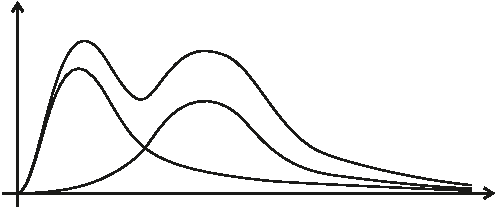
\includegraphics[width=0.6\linewidth]{pictures/8_1.pdf}
			\caption{no idea what is it and where did it come from :D....me neither :D}
			\label{fig:81}
		\end{figure}
		
\end{remark}

\chapter{Nejméně příznivá apriorní rozdělení, souvislost s~minimaxním principem rozhodování.}

\section{Propojování Bayesovské statistiky s klasickou statistikou (nejméně příznivé rozdělení)}
\begin{define}
	Mějme $\t\in\Theta,~\tau(\t)\in\mathcal{T}$, rozhodovací prostor (\textit{decision space}) $\Dd $, ztrátovou funkci  $L(\t,\delta)$ ($\delta_L$ $\forall \t,\forall \textbf{x}$), rizikovou funkci $\RF(\t,\delta)=\E^fL$ ($\delta_U$ $\forall\t$) a supremální rizikovou funkci $\sup_\t\RF(\t,\delta)$ ($\delta_0$). Dále ÚBM a apriorní bayesovské riziko $r(\pi,\delta)=\E^\pi\RF(\t,\delta)$ ($\delta^{\pi}=\argmin\limits_{\delta\in\Dd }r(\pi,\delta)$). Definujeme $\underline{\RF}=\sup\limits_{\pi\in\Pi} r(\pi,\delta^{\pi})=\sup\limits_{\pi\in\Pi}\inf\limits_{\delta} r(\pi,\delta)=\sup\limits_{\pi\in\Pi}r(\pi),$ kde $\Pi$ je rodina apriorních hustot a $\underline{\RF}$ nazveme maximinimální riziko.
\end{define}
\begin{theorem}\label{veticka}
	$\underline{\RF}\leq \overline{\RF}$, kde $\overline{\RF}=\inf\limits_\delta\sup\limits_\t \RF(\t,\delta)$ (minimaxní riziko).
	\begin{proof}
		Volme apriorní rozdělení $\pi$ $\Rightarrow$ $$ r(\pi,\delta)=\int_\Theta\underbrace{\RF(\t,\delta)}_{\geq0\wedge\leq \sup\limits_{\t}\RF(\t,\delta)}\underbrace{\pi(\t)}_{\geq0}\d\t\leq \int_{\Theta}\sup\limits_\t \RF(\t,\delta)\pi(\t)\d\t=\sup\limits_\t \RF(\t,\delta)\cdot \underbrace{1}_{\int_{\Theta}\pi(\t)\d\t}.$$
		Dále platí nerovnice \[
		\begin{split}
		r(\pi,\delta)&\leq \sup\limits_\t\RF(\t,\delta),\quad \forall\delta,\forall\pi\\
		\inf\limits_\delta r(\pi,\delta)&\leq \inf\limits_\delta\sup\limits_\t \RF (=\overline{\RF}),\quad \forall\pi\\
		\sup\limits_\pi\inf\limits_\delta r=\underline{\RF}&\leq \sup\limits_{\pi}\overline{\RF}=\overline{\RF}
		\end{split}
		\]
	\end{proof}
\end{theorem}
\begin{remark}
	Pokud $\delta^\pi$ dosahuje na $\underline{\RF}$ a $\underline{\RF}=\overline{\RF}$ ve větě \ref{veticka}, pak $\delta^\pi$ je současně \textbf{minimaxní strategie}.
\end{remark}
\begin{define}
	Pokud existuje $\pi^\ast$ apriorní rozdělení takové, že $r(\pi ^\ast)=\underline{\RF}$ (tzn. $\forall\pi\in\Pi,~r(\pi)\leq r(\pi^\ast)$), tak pak se nazývá \textbf{nejméně příznivé} (least favourable).
\end{define}

\begin{theorem}\label{veticka2}
	Nechť $\pi$ je vlastní apriorní rozdělení na $\Theta$ tak, že $r(\pi)=\sup\limits_\t\RF(\t,\delta^\pi)$. Pak \begin{enumerate}
		\item $\delta^\pi$ je minimaxní strategií,
		\item pokud $\delta^\pi$ jednoznačné Bayesovské řešení, pak $\delta^\pi$ je jednoznačná minimaxní strategie,
		\item $\pi$ je nejméně příznivé rozdělení (LF). 
	\end{enumerate}
\begin{proof}
	\begin{enumerate}
		\item Vezmeme $\delta$ libovolné fixní. Pak $\sup\limits_\t\RF(\t,\delta)\geq^{\text{\footnotemark}}\int\RF\pi(\t)\d\t=\E^\pi\RF=r(\pi,\delta)\geq r(\pi,\delta^\pi)=r(\pi)=\sup\limits_\t\RF(\t,\delta^\pi)$. \footnotetext{$\sup\limits_\t\RF(\t,\delta)\cdot 1=\sup\limits_\t\RF(\t,\delta)\int\pi(\t)\d\t$ $\wedge$ $\sup\limits_\t\RF(\t,\delta)\geq \RF$}
		\item Analogicky jako předchozí bod, akorát $r(\pi,\delta)> r(\pi,\delta^\pi)$
		\item Volíme $\pi'$ libovolné fixní. Pak $r(\pi')=r(\pi',\delta^{\pi'})\leq r(\pi',\delta^\pi)\leq \sup\limits_\t\RF(\t,\delta^\pi)=r(\pi)$. Potom $\pi$ ($=\pi^\ast$) je LF.
	\end{enumerate}
\end{proof}
\end{theorem}
\begin{remark}
Věta \ref{veticka2} je jednou z prvních vět o tom, jak za daných podmínek lze z Bayesovské strategie získat klasickou minimaxní strategii.
\end{remark}
\begin{dusl}\label{dusledek2}
	Věta platí, pokud $\RF(\t,\delta^\pi)$ je konstantní v $\t$ na $\Theta$ s.j. vzhledem k apriornímu rozdělení $\pi$, pak $r(\pi)=\sup\RF$.
\end{dusl}
\begin{theorem}
	Nejméně příznivá posloupnost $(\pi_n)_1^{+\infty}$ je taková, že $\exists\lim\limits_{n\to+\infty} r(\pi_n)=\underline{\RF}$. 
\end{theorem}
\begin{theorem}\label{veticka3}
	Nechť $(\pi_n)_1^{+\infty}$ je posloupnost taková, že $\lim\limits_{n\to+\infty}r(\pi_n)=r$. Nechť $\delta_0$ je libovolná rozhodovací funkce taková, že $\sup\limits_\t \RF(\t,\delta_0)=r$. Pak \begin{enumerate}
		\item $\delta_0$ je minimaxní,
		\item NELZE VYSLOVIT
		\item $(\pi_n)_1^{+\infty}$ je nejméně příznivá posloupnost apriorních rozdělení (LF).
	\end{enumerate}
\begin{proof}
	Analogicky jako ve větě \ref{veticka2} (tedy za domácí cvičení).
\end{proof}
\end{theorem}
\begin{example}
	Mějme $X\sim \mathrm{Bi}(n,p),~\widehat{p}=?,~\pi(p)\sim\mathrm{Beta}(a,b)\sim\frac{1}{B(a,b)}p^{a-1}(1-p)^{b-1}$, kde $a,b>0$. Příkladem může být teorie spolehlivosti, kde máme datové pole v RAIDu, tj. $n$ komponentní systém. Označme $X$ počet poruch za čas $1$. Pokud nastane jev $\{X\geq5\}$, tak nastane výpadek. Jaká je pravděpodobnost $\PP(X\geq5)=\widehat{p}$. $\widehat{\E X}=n\widehat{p}$ za čas 1.
	
	Se zadáním můžeme dělat několik věcí:\begin{enumerate}[1)]
		\item apriorní odhad $\widehat{p}_a=\E\mathrm{Beta}(a,b)=\frac{a}{a+b}.$
		\item Můžeme naměřit data $x$ a vypočíst klasický odhad ML: $\widehat{p}_\mathrm{ML}=\frac{x}{n}=\oxnn$ (Pokud $(L=L_2)$, tak je to $\widehat{p}_\mathrm{UMVUE}$).
		\item Bayesovský odhad: $$\pi(p|x)=\frac{\binom{n}{x}p^x(1-p)^{n-x}\cdot\frac{1}{B(a,b)}p^{a-1}(1-p)^{b-1}}{\int_{0}^{1}-||-\d p}=\frac{1}{c}p^{x+a-1}(1-p)^{n-x+b-1}\sim\mathrm{Beta}(x+a,n-x+b).$$
		Z toho potom $\widehat{p}_\mathrm{B}=\E \mathrm{Beta}(x+a,n-x+b)=\frac{x+a}{n+a+b}=\frac{\oxnn+\frac{a}{n}}{1+\frac{a+b}{n}}$. Zároveň však lze $\widehat{p}_\mathrm{B}$ zapsat jako konvexní kombinaci z bodu 2)
		$$ \widehat{p}_\mathrm{B}=\underbrace{\frac{a+b}{a+b+n}}_{\alpha_n}\frac{a}{a+b}+\underbrace{\frac{n}{n+a+b}}_{1-\alpha_n}\frac{x}{n}=\alpha_n\widehat{p}_a+(1-\alpha_n)\widehat{p}_\mathrm{ML},$$ kde $\alpha_n$ se nazývá porce neurčitosti apriorní znalosti.
		\begin{enumerate}[a)]
			\item $n$ pevně, $a,b\to+\infty$ (velké), $b/a=konst$ $(\alpha_n\to1\Rightarrow\widehat{p}_\mathrm{B}=\widehat{p}_a)$
			\item $a,b$ pevně, $n\to+\infty$ (velké), pak $\alpha_n\to0$ $(\alpha_n\doteq0)\Rightarrow\widehat{p}_\mathrm{B}=\widehat{p}_\mathrm{ML}$,
			\item $a=b=1$, tzn. $\pi(p)=U(0,1)$ - princip neurčitosti. Z toho pak $\widehat{p}_\mathrm{B}=\frac{x+1}{n+2}\doteq \widehat{p}_\mathrm{ML}$ pro vysoká $n$.
			\item $a=b=0,~\pi(p)=\inv{p}\inv{(1-p)}$ je apriorní nevlastní limitní rozdělení, pak $\pB=\pML$.
			\item $a=a_n=\frac{\sqrt{n}}{2},~b=b_n=\frac{\sqrt{n}}{2}$, tzn. $\pi(p)=\mathrm{Beta}\big(\frac{\sqrt{n}}{2},\frac{\sqrt{n}}{2}\big)$ (závisí na $n$).
			\[
			\begin{split}
			\pB&=\frac{x+\frac{\sqrt{n}}{2}}{n+\sqrt{n}}\Rightarrow \RF(p,\pB)=\Big|L=L_2\Big|=\E \underbrace{(p-\widehat{p}_\mathrm{B})^2}_{L_2(p,\pB)}=\E\Big(p-\frac{X+\frac{\sqrt{n}}{2}}{n+\sqrt{n}}\Big)^2=\\&=c\underbrace{\E X^2}_{np-np^2+n^2p^2}+d \underbrace{\E X}_{np}+e=\dots=\frac{n}{4(n+\sqrt{n})^2}=konst.
			\end{split}
			\] 
			Dle věty \ref{veticka2} a důsledku \ref{dusledek2} víme, že $r(\pi)=\sup\limits_{\theta}\RF(\t,\delta^\pi)$ implikuje to, že $\pB~=~\widehat{p}_\mathrm{Minimax}$ a $\pi^\ast=\pi(p)$ je LF.
			\begin{figure}[h]
				\centering
				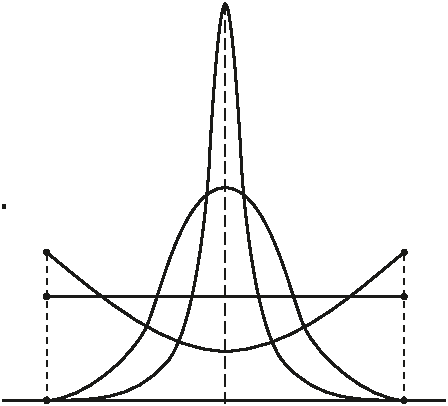
\includegraphics[width=0.5\linewidth]{pictures/9_1.pdf}
				\caption{popis}
				\label{fig:91}
			\end{figure}			
		\end{enumerate}
	\end{enumerate}
\end{example}	
	
\begin{example}
	Mějme $X\sim\NN(\mu,1)=\NN(\t,1),~\wmu=?$, $x$ data $\Rightarrow$ $\widehat{\mu}_{\mathrm{ML}}=x(=\overline{x}_n)$
	\begin{enumerate}[A)]
		\item Zvolíme neurčitou informaci $\pi(\mu)=konst=1$ na $\R$ nevlastní ($\wmu_a$ není). $$\pi(\mu|x)=\frac{1}{\sqrt{2\pi}}\e{-\frac{1}{2}(x-\mu)^2}\cdot \frac{1}{\int_\R -||-\d\mu}=\frac{1}{\sqrt{2\pi}}\e{-\frac{1}{2}(\mu-x)^2}\sim\NN(x,1).$$
		$$\widehat{\mu}_\mathrm{B}=\EE{\NN(x,1)}=x(=\oxnn),$$
		$$ \RF(\mu,\widehat{\mu}_\mathrm{B})\equal{L=L_2}\E(\mu-X)^2=\D X=1,$$ tzn. $\RF(\mu,\widehat{\mu}_\mathrm{B})=konst.$, ale nelze aplikovat větu \ref{veticka2}, protože $\pi$ není vlastní.
		\item $\pi_n(\mu)=\NN(0,n)$ je vlastní hustota $\forall n$ (CF)(zkusíme na větu \ref{veticka3}).
		\[
		\begin{split}
		\pi_n(\mu|x)~\propto~ \e{-\frac{1}{2}(x-\mu)^2}\e{-\frac{1}{2n}(\mu-0)^2}~\propto~\e{-\frac{1}{2}\big[\big(1+\frac{1}{n}\big)\mu^2-2\mu x+x^2\big]}~\propto~\e{-\frac{1}{2}\big(1+\frac{1}{n}\big)\big[\mu-\frac{n}{n+1}x\big]^2}\sim \NN\Big(\frac{n}{n+1}x,\frac{n}{n+1}\Big)
		\end{split}
		\]
		$$\widehat{\mu}_\mathrm{B}=\E \NN\Big(\frac{n}{n+1}x,\frac{n}{n+1}\Big)=\frac{n}{n+1}x=\delta^{\pi_n}\sim\widehat{\mu}_{B,n}.$$
		$$r(\pi_n)\equal{L=L_2}\D \pi(\mu|x)=\frac{n}{n+1}\to1 \text{ (ověříme vzorec v následující větě)}.$$
		$\lim\limits_{n\to+\infty}r(\pi_n)=1=r$ a víme, že máme $\delta_0$, pro který je $r=\RF(\mu,\underbrace{\overbrace{\widehat{\mu}_\mathrm{B}}^{\text{z A)}}}_{=\delta_0=x})$. Potom dle věty \ref{veticka3} je $\delta_0=x$ minimaxní a posloupnost $\NN(0,n)$ je LF. (V tomto příkladu jsme používali $\propto$ (úměrnost), protože jsme nijak neřešili konstanty)
	\end{enumerate}
\end{example}
\begin{theorem}[!!!Vyhazovací!!!]\label{vyhazovaci}
	ÚBM, $X\sim f(x|\t),~\pi(\t),~L(\t,\delta)=L_2(\t,\delta)=(\t-\delta)^2$. Nechť pro aposteriorní střední hodnotu platí, že $0<\E^\pi(\t^2|x)<+\infty$ ($\neq 0$ aby nebyla degenerovaná). Pak $$\delta^\pi(x)=\E^\pi(\t|x)=\frac{\int\t f(x|\t)\pi(\t)\d\t}{\int f(x|\t)\pi(\t)\d\t}, \text{ , kde } \frac{f(x|\t)\pi(\t)}{\int f(x|\t)\pi(\t)\d\t}=\pi(\t|x)$$
	a Bayesovské riziko 
	$$r(\pi)=\E^m[\D^\pi(\t|x)],$$
	kde $m(x)=\int f\pi\d\t$.
	\begin{proof}
	Vyjdeme z definice bayesovského odhadu $\delta^\pi=\argmin\limits_{\delta} r(\pi,\delta)$
		\[
		\begin{split}
		r(\pi,\delta)&=\E^\pi[\RF(\t,\delta)]=\E^\pi\big[\E^f\big(\t-\delta(X)\big)^2\big]=\left|\begin{array}{c}
		\text{záměna} \\ \E^\pi\text{ a }\E^f		
		\end{array}
		\right|=\E^m\big[\E^\pi\big(\t-\delta(x)\big)^2\big|x\big]=\\&=\E^m\big[\E^\pi(\t^2|x)-2\delta(x)\E^\pi(\t|x)+\delta(x)^2\big]=\E^m\big[\underbrace{\E^\pi(\t^2|x)}_{0<...<+\infty}+\big(\delta(x)-\E^\pi(\t|x)\big)^2-\underbrace{\big(\E^\pi(\t|x)\big)^2}_{0<...<+\infty}\big]
		\end{split}
		\] Abychom tento výraz optimalizovali, musíme vzít $\delta^{\pi}=\delta(x)=\E^\pi(\t|x)$, abychom výraz minimalizovali.
		$$ r(\pi)=r(\pi,\delta^\pi)=\E^m\big[\underbrace{\E^\pi\big(\t-\E^\pi(\t|x)\big)^2|x}_{\D(\t|x)}\big].$$
		Záměna je provedena obdobně jako ve větě \ref{veta_zamena}.
	\end{proof}
\end{theorem}

\chapter{Přípustnost bayesovského řešení, Steinův efekt pro~sféricky symetrická rozdělení, Bergerův jev.}

\section{Přípustnost (Admissibility)}
\begin{define}
	Mějme $\Dd ,\Theta,...$ Rozhodovací funkce $\delta_0$ se nazývá \textbf{nepřípustná}, pokud existuje $\delta_1$, která dominuje $\delta_0$, ozn. $\delta_1\ll\delta_0$, tzn. $\RF(\t,\delta_1)\leq\RF(\t,\delta_0),~\forall\t\in\Theta$ (stejnoměrně) a $\exists\t_0\in\Theta$ tak, že $\RF(\t_0,\delta_1)<\RF(\t_0,\delta_0)$. V případě, že taková $\delta_1$ neexistuje, pak $\delta_0$ nazýváme \textbf{přípustný}.
	
	\begin{figure}[h]
		\centering
		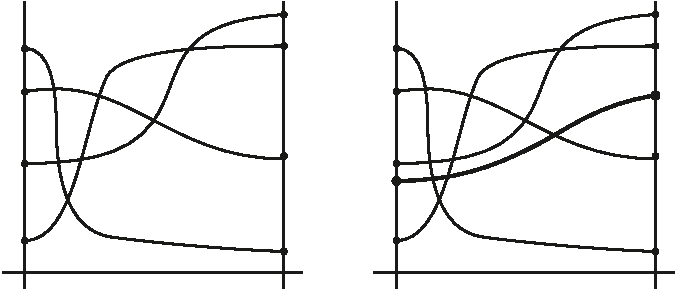
\includegraphics[width=0.6\linewidth]{pictures/9_2-3.pdf}
		\caption{Který je přípustný? Všechny 4. Vpravo ale už je $\RF(\t,\delta_\circ)$ nepřípustný.}
		\label{fig:92}
	\end{figure}
	\FloatBarrier
	
\end{define}
\begin{theorem}\label{veta_pripustna}
	\begin{itemize}
		%\item 	$\delta_L(x)=\argmin\limits_\delta L\big(\t,\delta(x)\big),~\forall\t,\forall x$, je vždy přípustný, pokud existuje, 
	\item  $\delta_U=\argmin\limits_\delta\RF(\t,\delta),~\forall\t$, je vždy přípustný, pokud existuje, \item  $\delta_0=\argmin\limits_\delta\sup\limits_\t\RF(\t,\delta)$ je přípustný, pokud existuje a je jednoznačný, \item  $\delta^\pi=\argmin\limits_\delta r(\pi,\delta)$ je přípustný, pokud existuje a je jednoznačný.
\end{itemize}
\end{theorem}


%%% 26.11.2020

\begin{theorem}\label{veta_rovnost}
	Nechť $L(\t,\delta)$ je striktně konvexní v $\delta$ pro $\forall\t$. Mějme $\delta_0$ rozhodovací funkci pro $\tau(\t)/(\t)$ a $\delta_0$ je přípustný. Nechť $\delta'$ je tak, že $\RF(\t,\delta')=\RF(\t,\delta_0),~\forall\t$. Pak $\delta'=\delta_0$ s pravděpodobností 1 ($s.j.$), tedy $$ \E L(\t,\delta'(X))=\E L(\t,\delta_0(X)).$$
	\begin{proof}
		Sporem: $\delta_0\neq\delta'$ s nenulovou pravděpodobností. Sestrojíme $\delta^\ast=\frac{\delta_0+\delta'}{2}$ (konvexní kombinace). Pak
		\[
		\begin{split}
		\RF(\t,\delta^\ast)&=\E L\big(\t,\delta^\ast(X)\big)=\E\Big[L\Big(\t,\frac{\delta_0+\delta'}{2}\Big)\Big]\overset{\forall\t}{<}\E\Big[\frac{1}{2}L(\t,\delta_0)+\frac{1}{2}L(\t,\delta')\Big]=\\&= \frac{1}{2}\underbrace{\E L(\t,\delta_0)}_{\RF(\t,\delta_0)}+\frac{1}{2}\underbrace{\E L(\t,\delta')}_{\RF(\t,\delta')=\RF(\t,\delta_0)\,\forall\t}=\RF(\t,\delta_0),~\forall\t.
		\end{split}
		\] 
		To znamená, že $\delta^\ast\ll\delta_0$, což je spor s přípustností $\delta_0$.
	\end{proof}
\end{theorem}
\begin{theorem} \label{veta_prip}
	Jednoznačná $\delta^\pi$ je vždy přípustná riziková funkce, pokud existuje. (Část věty \ref{veta_pripustna})
	\begin{proof}
		$\delta^\pi$ jednoznačný Bayes, pak \[
		\begin{split}
		r(\pi,\delta^\pi)&<r(\pi,\delta),\quad\forall\delta,\\
		\E \RF(\t,\delta^\pi)&<\E \RF(\t,\delta),\quad\forall\delta,\\
		\int\RF(\t,\delta^\pi)\pi(\t)\d\t&<\int\RF(\t,\delta)\pi(\t)\d\t,\quad\forall\delta.		
		\end{split}
		\]
		Z toho vyplývá, že $\exists\t_0$, $\RF(\t_0,\delta^\pi)<\RF(\t_0,\delta),~\forall\delta$. Kvůli tomu $\delta$ nedominuje $\delta^\pi$, a proto je $\delta^\pi$ přípustná.
	\end{proof}
\end{theorem}
\begin{remark}
	Pokud $L(\t,\delta)$ je striktně konvexní v $\delta$ pro $\forall\t$, pak $\delta^\pi$ je vždy jednoznačná.
\end{remark}
\begin{theorem}
	ÚBM, $X\sim f(x|\t),~\pi(\t)$. Nechť $\pi(\t)>0$ pro $\forall\t$, nechť dále $\delta^{\pi}$ existuje a $r(\pi)=r(\pi,\delta^{\pi})<+\infty$. Nechť $\RF(\t,\delta)$ je spojitá v $\t$ pro $\forall \delta$. Pak $\delta^\pi$ je přípustná. (Větu lze ukázat i pro $r(\pi,\delta^{\pi})=+\infty$)
	\begin{proof}
		Sporem. Nechť $\delta^\pi$ je nepřípustná. Pak by ale $\exists\delta_0\ll\delta^\pi$, tzn. $\RF(\t,\delta_0)$ stejnoměrně vylepšuje $\RF(\t,\delta^\pi)$ a $\exists\t_0$ tak, že $\RF(\t_0,\delta_0)<\RF(\t_0,\delta^\pi)$,viz obr. \ref{fig:26}.
		\begin{figure}[h]
			\centering
			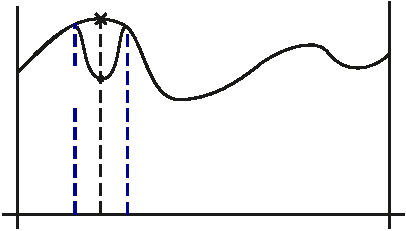
\includegraphics[width=0.35\linewidth]{pictures/26_11.pdf}
			\caption{popis}
			\label{fig:26}
		\end{figure}
		Potom by ale existovalo okolí $H_{\t_0}$ tak, že $\RF(\t,\delta_0)<\RF(\t,\delta^\pi)$ na $H_{\t_0}$. Potom by platilo, že $\E^{\pi} \RF(\t,\delta_0)<\E^\pi \RF(\t,\delta^\pi)$. To platí, protože $\pi(\t)>0,~\forall\t$. Potom tedy 
		$$ r(\pi,\delta_0)<\underbrace{r(\pi,\delta^\pi)}_{r(\pi)<+\infty},$$ což je spor s tím, že $\delta^{\pi}$ je Bayesovská strategie. (V $\delta^{\pi}$ dosahuje minima a my jsme našli menší)
	\end{proof} 
\end{theorem}
\begin{remark}[Komentář k předpokladům předchozí věty]
	$\pi(\t)>0$
\begin{enumerate}[a)]
	\item 	\begin{center}
			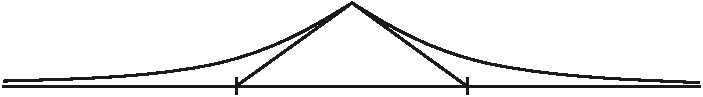
\includegraphics[width=0.7\linewidth]{pictures/26_11_2.pdf}
	\end{center}
\item $\RF(\t,\delta)=\E L\big(\t,\delta(X)\big)=\int_{\chi(\R^n)}L\big(\t,\delta(x)\big)f(x|\t)\d x$. Zde stačí zajistit, aby měl integrand Lebegovskou majorantu, protože chceme $L$ spojitou v $\t$.
\end{enumerate}

\end{remark}
\begin{remark}
	Doteď jsme dělali, že $\delta^{\pi}\overset{podm.}{\Rightarrow}$ přípustné. Lze tuto implikaci obrátit? 
	\begin{description}
		\item[Stein (1955+)] Nutná a postačující podmínka, ze které jsou všechny přípustné rozhodovací funkce limitami posloupnosti $\delta^{\pi_n}$ Bayesovských strategií.
		\item[Farrell (1968)] Předpokládáme, že \begin{enumerate}[1)]
			\item $f(x|\t)$ spojitá v $\t$, $f>0$ na $\Theta$,
			\item $L(\t,\delta)$ je striktně konvexní, spojitá,
			\item $\forall E\subset\Theta$ kompaktní platí, že 
			$$ \lim\limits_{\left\|\delta\right\|\to+\infty}\inf\limits_{\t\in E}L(\t,\delta)=+\infty.\qquad(\text{L je nutně neomezená funkce})$$ 
		\end{enumerate}
	Pak libovolná $\delta_0$ přípustná je limitou $\delta^{\pi_n}$ Bayesovských strategií.
	\item[Brown (1986)] Předpokládejme, že \begin{enumerate}[1)]
		\item $L$ striktně konvexní,
		\item $f(x|\t)>0$, $\Dd $ uzavřená a konvexní,
		\item $L$ je zdola polospojitá (lower semicontinuous), tzn. $f$ je v $x_0$ zdola polospojitá, pokud $(\forall\epsilon>0)(\exists H_{x_0})\big(f(x)\geq f(x_0)-\epsilon\big)$ na $H_{x_0}$.
		\item $\lim\limits_{\left\|\delta\right\|\to+\infty} L(\t,\delta)=+\infty$ \hspace{0.2cm} ($L$ je nutně neomezená funkce).
	\end{enumerate}
Pak libovolná přípustná strategie je bodovou limitou $\delta^{\pi_n}$ Bayesovské posloupnosti, kde $\pi_n(\t)$ mají omezený support.
\item[Závěr] Libovolná přípustná strategie $\delta$ je dosažitelná buď přímo Bayesovským odhadem $\delta^\pi$ nebo zobecněným Bayesovským odhadem $\delta^\pi$, nebo posloupností $\delta^{\pi_n}$.
	\end{description}
\end{remark}
Jak funguje přípustnost u klasických statistických strategií?
\begin{theorem}\label{veta_mini}
	Pokud existuje jednoznačně minimaxní strategie $\delta_0$, pak je přípustný.\begin{proof}
		Ponecháno čtenáři. (Obdobně jako ve větě \ref{veta_prip})
	\end{proof}
\end{theorem}
\begin{theorem}["Obrátka"]
	Nechť $L(\t,\delta)$ je striktně konvexní v $\delta$ pro $\forall\t$, $\delta_0$ je přípustná rozhodovací funkce a $\delta_0$ má konstantní riziko $\RF$. Pak $\delta_0$ je jednoznačná minimaxní strategie.
	\begin{figure}[h]
		\centering
		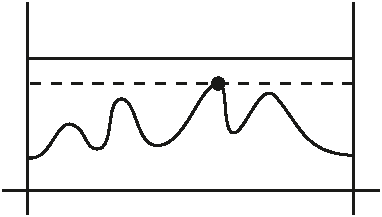
\includegraphics[width=0.4\linewidth]{pictures/26_11_3.pdf}
		\caption{popis}
		\label{fig:26-3}
	\end{figure}
	
	\begin{proof}
		\begin{enumerate}[1)]
			\item Ukážeme, že $\delta_0$ je minimaxní - sporem: $\delta_0$ není minimax, viz obrázek \ref{fig:26-3}. Konstantní $\RF(\t,\delta_0)\Rightarrow$ pod ní funkce $\RF(\t,\delta_1)\Rightarrow$ ta vylepšuje odhad $\RF(\t,\delta_0)$, což je spor s přípustností $\delta_0$.
			\item Jednoznačnost - $\delta_0$ je minimax: sporem. $\exists\delta_1\neq\delta_0$ a přitom $\delta_1$ je minimaxní.
			\begin{enumerate}[a)]
			\item $\RF(\t,\delta_0)=\RF(\t,\delta_1)\,\forall\t$. Ihned získáváme spor díky větě \ref{veta_rovnost} ($\delta_0=\delta_1$ s.j.)
			\item $\RF(\t,\delta_0)$ konstantní z předpokladu a $\RF(\t,\delta_1)$ je pod ní, ale mají stejné supremum, což je spor s přípustností $\delta_0$, protože jsme našli $\delta_1$ takovou, že $\delta_1\ll\delta_0$
			\end{enumerate}
			\begin{center}
				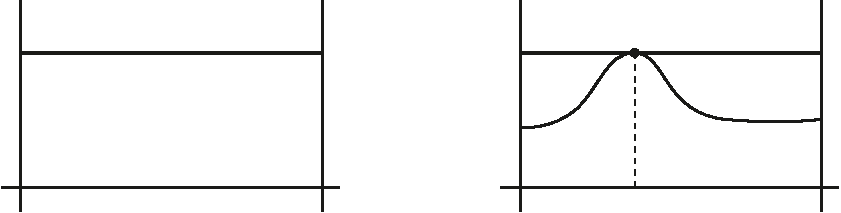
\includegraphics[width=0.7\linewidth]{pictures/26_11_4.pdf}
			\end{center}
		\end{enumerate}
	\end{proof}
\end{theorem}
\subsection{Steinův efekt (paradox) (1955)\,[Stejnův]}
Nechť $\textbf{X}\sim f(\textbf{x},\boldsymbol{\t}),~\boldsymbol{\t}\in\Theta\subset\R^k,~f$ je sféricky symetrické rozdělení okolo $\boldsymbol{\t}$, tzn. $f(\left\|\textbf{x}'-\boldsymbol{\t}\right\|+\left\|\textbf{x}''\right\|)$, kde $\textbf{x}=(\textbf{x}',\textbf{x}''),~\textbf{x}'\in\R^k,~\textbf{x}''\in\R^{n-k}$ (např. $\NN_k(\boldsymbol{\t},\I_{k\times k})$). Volme pro $\boldsymbol{\t}$ váženou kvadratickou ztrátovou funkci $L_2^w(\boldsymbol{\t},\boldsymbol{\delta})=\sum_{j=1}^k w_j\cdot(\t_j-\delta_j)^2$. 
	
Označme $\boldsymbol{\delta}^\ast(\textbf{x})=\big(\delta_1^\ast(\textbf{x}),...,\delta_k^\ast(\textbf{x})\big)$ odhad (rozhodovacích funkcí) pro $\boldsymbol{\t}$ získaný klasickou statistickou procedurou. 

Pak $\exists k_0$ tak, že $\forall k\geq k_0$ je $\boldsymbol{\delta}^\ast$ nepřípustným odhadem (rozhodovací funkce) pro $\boldsymbol{\t}$, přestože $\delta_j^\ast$ jsou pro odhad $\t_j$ přípustné $\forall j\in\widehat{k}$.
\begin{dusl}
	Například klasická rozhodovací funkce metodou jednoznačného minimaxu je od jistého $k_0$ beznadějná, protože víme (z věty \ref{veta_mini}), že pokud existuje jednoznačný minimax, pak je přípustný. Stein ale říká, že od jistého $k_0$ se klasickou statistickou procedurou získat přípustné řešení nedá, tzn. od jistého $k_0$ nemůže existovat jednoznačný minimax. A také stejnoměrně nejlepší strategie $\delta_U$ od jisté dimenze $k_0$ neexistuje.
\end{dusl}
Co s tím? Místo $\delta_u=\argmin\limits_{\delta\in\Dd }\RF(\t,\delta),~\forall\t$ hledá $\delta_{pu}=\argmin\limits_{\delta\in\Dd _0\subset\Dd }\RF(\t,\delta)\,\forall\t$, např. $\Dd _0$ nestranné odhady (UMVUE). Tím jsme zajistili existenci, ale pro vysokou dimenzi opět dostaneme nepřípustné řešení. Další možností je použít $\Dd _0'$ jako \textbf{ekvivariantní} odhady. Ty pak vedou na UMEqE (\textit{Uniformly minimum equivariant estimator}).  

Řešení se pak nabízí v podobě Bayese (začlenění apriorní informace $\pi$).

\begin{description}
	\item[1955 Steinův efekt:] Mějme $X\sim \NN_k(\boldsymbol{\t},\mathbb{I}_{k\times k})$ a nechť $\delta_0(\textbf{x})=\textbf{x}$ je ML, minimaxní a víme, že $\RF(\t,\delta_0)=konst$. Do roku 1955 se myslelo, že $\delta_0$ je jednoznačný minimax $\forall k$. Dle věty o jednoznačnosti minimaxu by bylo $\delta_0$  přípustné $\forall k$. Stein však roku 1955 ukázal, že $\delta_0$ je jednoznačný minimax a přípustný pro $k=1,2$ a že pro $(\forall k\geq3)(\exists\delta')(\delta'\ll\delta_0)$.
	  \begin{figure}[h]
		\centering
		\begin{asy}
		unitsize(0.65cm);
		arrowbar myarrow=Arrow;
		void xtick(real x){draw((x,-.1) -- (x,.1));}
		
		void ytick(real y){draw((-.1,y) -- (.1,y));}
		
		path s = ((0,.5) .. (1.5,1.2) .. (3,2) .. (4.5,1.2) .. (6,.5) .. (7,.4));
		draw(s);
		draw((-.1,0) -- (7.1,0));
		draw((0,-.1) -- (0,3));
		draw((6,-.1) -- (6,3));
		dot((3,2));
		draw((0,2)--(7,2));
		ytick(2);
		label("$\mathrm{R}(\theta,\delta_0)$",(3,2.5));
		label("$\left\|\theta\right\|$",(3,-0.5));
		\end{asy}
		\caption{Popis.}\label{pic2}
	\end{figure}
	\FloatBarrier
	\item[1961 James-Steinův (shrinkable) odhad parametru polohy:]$$ \delta^\mathrm{JS}(\textbf{x})=\underbrace{\Big(1-\frac{k-2}{\left\|\textbf{x}\right\|^2}\Big)}_{\to-\infty\text{ při }\left\|\textbf{x}\right\|\to0^+}\cdot\textbf{x} $$
	\item[1970 Baranchick:] $$ \delta_c^+\cdot(\textbf{x})=\Big(1-\frac{c}{\left\|\textbf{x}\right\|^2}\Big)^+\textbf{x}=\begin{cases}
	\big(1-\frac{c}{\left\|\textbf{x}\right\|^2}\big)\textbf{x} & \text{pokud }c<\|\textbf{x}\|^2 \\0 & \text{jinak,}
	\end{cases} $$
	kde $c\in\langle k-2,2(k-2)\rangle$. Pak $\delta_c^+\ll \delta_\mathrm{JS} \ll \delta_0,~\forall k\geq 3$.
	\item[1994 Shao et al.] $\exists \delta_S \ll \delta_c^+$, ale vylepšení už nestojí za tu složitost (tedy Baranchick je kompromis v rámci použitelnosti).
\end{description}
\begin{remark}
   Pro $c=2k-1\notin \langle k-2,2(k-2)\rangle$ je Baranchickova, ale nedominuje $\delta_{JS}$, $\RF(\t,\delta_{2k-1}^+)$.
   \begin{figure}[h]
   	\centering
   	\begin{asy}
   	unitsize(0.65cm);
   	arrowbar myarrow=Arrow;
   	void xtick(real x){draw((x,-.1) -- (x,.1));}
   	
   	void ytick(real y){draw((-.1,y) -- (.1,y));}
   	
   	path s = ((0,1) .. (2,2.2) .. (4,2.1) .. (6,2));
   	draw(s);
   	draw((-.1,0) -- (7.5,0), arrow=myarrow);
   	draw((0,-.1) -- (0,3), arrow=myarrow);
   	draw((0,2)--(6,2));
   	ytick(2);
   	label("$\mathrm{R}(\theta,\delta_{2k-1}^+)$",(2,0.8));
   	label("$\left\|\theta\right\|$",(8.2,0));
   	label("$\big(\delta_0(\textbf{x})=\textbf{x}\big)~\mathrm{R}(\theta,\delta_0)$",(9,2));
   	label("$k$",(-0.4,2));
   	\end{asy}
   	\caption{Popis.}\label{pic1}
   \end{figure}
\end{remark}
\begin{theorem}[Bergerův jev]
	$\forall k_0\in\N$ (dimenzi $\boldsymbol{\t}$), existuje ztrátová funkce $L(\boldsymbol{\t},\boldsymbol{\delta})$ taková, že libovolný odhad $\boldsymbol{\delta}^\ast(\textbf{x})$ klasickou statistickou procedurou je $\forall k\geq k_0$ nepřípustný.
\end{theorem}

\begin{remark}
	Připomínka Rao-Blackwellovy věty: Mějme $L(\t,\delta)$ konvexní v $\delta$ pro $\forall\t$, $\textbf{T}(\textbf{X})$ je postačující statistika, $\delta_0$ je libovolná rozhodovací funkce. Pak $\widehat{\delta}(\textbf{t})=\EE{\delta_0(\textbf{X})|\textbf{T}(\textbf{X})=\textbf{t}}\ll \delta_0$ a $\E\widehat{\delta}=\E \delta_0$.
\end{remark}
\begin{define}
	Označme ztrátovou funkci $L\big(\t,\delta|\tau(\t)\big)$. Pak rozhodovací funkci $\delta(\textbf{x})$ nazýváme \textbf{nestrannou} vzhledem k $L$, pokud $$ \E L\big(\t,\delta|\tau(\t)\big)\leq \E L\big(\t,\delta|\phi(\t))\big),~\forall\phi,\forall\t.$$
\end{define}
Omezili jsme se na $\Dd _0\subset \Dd $ prostor nestranných rizikových funkcí vzhledem k $L$. Dále
$ \delta_U^0~=~\argmin_{\delta\in\Dd _0}\RF(\t,\delta),~\forall\t$ jako UBU$_L$E (\textit{Uniformly best unbiased estimators}), pokud existuje. Pak
$$ L=L_2(\t,\boldsymbol{\delta})=(\t-\delta)^2\equal{\text{případně}}\big(\tau(\t)-\delta\big)^2\quad\Rightarrow\quad UMVUE.$$

\begin{theorem}
	Mějme $L$ konvexní v $\delta$, $T(\textbf{X})$ je úplná postačující statistika, $\delta_0$ nestranná rozhodovací funkce vzhledem k $L_2$. Pak $\widehat{\delta}_\mathrm{R-B}(\textbf{t})$ je UMVUE (potenciálně nepřípustný (Stein)).
	
	\begin{figure}[h]
		\centering
		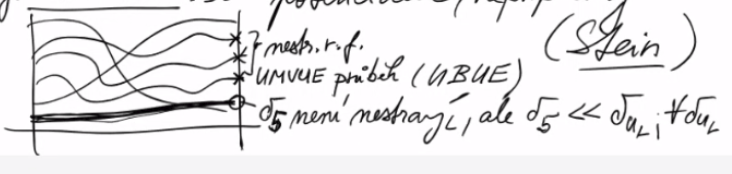
\includegraphics[width=0.6\linewidth]{pictures/3.12-1}
		\caption{popis}
		\label{fig:3}
	\end{figure}
	
\end{theorem}

\chapter{Grupy transformací, ekvivariantní odhady a~jejich bayesovská reprezentace.}

\section{Equivariantní rozhodovací funkce (MRE$_q$E)}
\begin{define}
	Mějme grupu $(G,\ast)$, tj. $g_1,g_2\in G~\Rightarrow~ g_1\ast g_2$ a volme speciálně grupu $(\R,\ast)$, \[
	\begin{split}
	g\in G,~x\in \R&~\Rightarrow g\ast x \\ \textbf{x}\in\R^n&~\Rightarrow~ g\ast \textbf{x}\text{ po složkách }\textbf{x},~\forall g\in G.
	\end{split}
	\]
	Vezmeme pravděpodobnostní model $X_j=\t\ast \epsilon_j$, kde $\epsilon_j$ značí chyby měření s $\epsilon_j\sim \PP_{0j},~\forall j\in\hat{n}$. $\textbf{X}=(X_j)_{j=1}^n=\t\ast\boldsymbol{\epsilon}$, kde $\boldsymbol{\epsilon}$ je chyba měření s $$\boldsymbol{\epsilon}\stackrel{id}{\sim}\prod_{j=1}^n \PP_{0j}\equal{iid}(\PP_{01})^n.$$
	Dále platí, že $$ \textbf{X}\sim \PP_\t\in\mathcal{P}_\ast=\{\PP_\t:\t\in\Theta\subset \R\}, g\in G~\Rightarrow~ g\ast \textbf{X}=g\ast(\t\ast\boldsymbol{\epsilon})=(g\ast\t)\ast\boldsymbol{\epsilon}\sim \PP_{g\ast \t}\in \mathcal{P}_\ast.$$ 
\end{define}
\begin{define}
	Rozhodovací funkce $\delta$ se nazývá \textbf{ekvivariantní} pro $\t$ vzhledem ke grupě $(G,\ast)$, pokud platí, že $$ \delta(g\ast\textbf{x})=g\ast \delta(\textbf{x}),\quad \forall g\in G,~\forall \textbf{x}\in\chi(\R^n).$$
\end{define}
\begin{define}
	Ztrátová funkce $L(\t,\delta)$ se nazývá \textbf{invariantní} vzhledem ke grupě $(G,\ast)$, pokud $$ L(g\ast\t,g\ast\delta)=L(\t,\delta)\quad\forall \t,\forall g,\forall \delta.$$
\end{define}
\begin{dusl}
	\[
	\begin{split}
	L(\t,\delta)\equal{\forall g}L(g\ast\t,g\ast \delta)&=\Big| \begin{array}{l}
	\text{volme }g=\widetilde{\t}\text{ inverzní prvek v }(G,\ast)\\\text{tzn. }\widetilde{\t}\ast\t=I/O\text{ neutrální prvek v }(G,\ast)
	\end{array}
	\Big|=L(\widetilde{\t}\ast\t,\widetilde{\t}\ast\delta)=\\&=L(I/O,\widetilde{\t}\ast\delta)=\rho(\widetilde{\t}\ast\delta),\quad\forall\t,\forall\delta.
	\end{split}
	\] 
\end{dusl}
\begin{dusl}
	\[
	\begin{split}
	\RF(\t,\delta)&=\E_\t L\big(\t,\delta(\textbf{X})\big)\equal{inv.~L}\E_\t\rho\big(\widetilde{\t}\ast\delta(\textbf{X})\big)=\Big|\begin{array}{l}
	\textbf{X}=\t\ast\boldsymbol{\epsilon}\\\boldsymbol{\epsilon}\sim\PP_0	
	\end{array}
	\Big|=\E_{\PP_0}\rho\big(\widetilde{\t}\ast\delta(\t\ast\boldsymbol{\epsilon})\big)\equal{\delta~ekvi.}\\&=\E_{\PP_0}\rho\big(\widetilde{\t}\ast\t\ast\delta(\boldsymbol{\epsilon})\big)=\E_{\PP_0}\rho\big(I/O\ast\delta(\boldsymbol{\epsilon})\big)=konst~v~\t,~\forall\t,
	\end{split}
	\]
tedy nezávisí na $\t$.
\end{dusl}
\begin{define}
	Definujeme $$ \delta^\ast:=\argmin_{\delta\in\Dd _{Eq}}\RF(\t,\delta),~\forall\t\quad-\text{říkáme }MRE_qE\,(\text{\textit{Minimum risk equivariant estimator}}).$$
\end{define}
\begin{example}
	Volme $(G,\ast)=(\R,+)$, $g\ast\textbf{x}=(x_1+g,...,x_n+g)=g+\textbf{x}.$ Pravděpodobnostní model se nazývá model s měřítkem (\textit{Location family}) (např. $\NN(\mu,\sigma^2 \text{ známé}))$
	\[
\begin{split}
X_j&=\t+\epsilon_j\quad(\text{aditivní chyba})\\
\textbf{X}&=\t+\boldsymbol{\epsilon}\sim\PP_\t\text{ a platí, že }\\
g\ast \textbf{X}&=g+\textbf{X}\sim \PP_{g+\t}.
\end{split}
\]
	$\delta$ je ekvivariantní, pokud $\delta(g+\textbf{x})=g+\delta(\textbf{x})$, např. $\delta(\textbf{x})=\frac{1}{n}\sumjn X_j$ (nebo také $\delta(\textbf{x})=x_{\text{medián}}$) je ekvivariantní rozhodovací funkce, protože $\delta(g+\textbf{x})=\frac{1}{n}\sumjn (X_j+g)=\frac{1}{n}\sumjn X_j + g=\delta(\textbf{x})+g$. $L$ invariantní znamená, že $L(\t,\delta)=\rho(\widetilde{\t}\ast\delta)=\rho(\delta-\t)\equal{\text{např.}}(\delta-\t)^2=L_2$. Máme tedy zajištěno, že $\RF(\t,\delta_{Eq})=konst.$ v $\t$.
\end{example}

Závěr: Existuje procedura pro hledání $MRE_qE$ pro $(G,\ast)=(\R,+)$ ve tvaru
$$ \delta^\ast(\textbf{x})=\argmin_{\delta\in\Dd _{Eq}}\frac{\int\rho(\delta-\t)f(\textbf{x}-\t)\d\t}{\int f(\textbf{x}-\t)\d\t}=\delta_\mathrm{B}^{\pi=1}(\textbf{x}).$$

\begin{remark}
	Připomínka: Bayesovské řešení $\widehat{\delta_\mathrm{B}}=\argmin_\delta r(\pi,\delta)$ nebo $\widehat{\delta_\mathrm{B}}(\textbf{x})= \argmin_{\delta(\textbf{x})}\rho(\pi,\delta|\textbf{x})$, kde $\rho(\pi,\delta|\textbf{x})$ se nazývá aposteriorní bayesovské riziko a splňuje (toto $\rho$ není to stejné jako v textu výše) 
	$$ \rho(\pi,\delta|\textbf{x})=\E^\pi[L|\textbf{x}]=\int L(\t,\delta)\pi(\t|\textbf{x})\d\t=\int L(\t,\delta)\frac{f \pi(\t)}{\int f \pi(\t)\d\t}\d\t.$$
 Zde stačí volit $\pi(\t)=1$ na $\Theta$ (potenciálně nevlastní). Pokud zvolíme konkrétně $L=L_2$, pak $\delta^\ast(\textbf{x})=\frac{\int\t f(\textbf{x}-\t)\d\t}{\int f(\textbf{x}-\t)\d\t}$, což se nazývá \textbf{Pitmanův odhad}.
\end{remark}
\begin{example}
	Mějme $\epsilon_j~\sim~iid~\mathrm{Exp}(1)$, $f(\textbf{x}-\t)=\e{-\sumjn x_j+n\t}$, pokud $\t< x_{(1)}~=~\min\big\{ (x_j)_1^n\big\}$. Dále pak
	$$ \delta^\ast(\textbf{x})\equal{L_2}...=x_{(1)}-\frac{1}{n},$$ což je Pitmanův odhad pro $\mathrm{Exp}(1)$, tedy $MRE_qE$.
\end{example}

\chapter{Bayesovské odhady pro~absolutní, multi-lineární, (váženou) kvadratickou a~0-1 ztrátovou funkci.}
%########################## LESSON 10.12
\begin{theorem}[Opakování vyhazovací věty \ref{vyhazovaci}]\label{veta1}
	Mějme $X\sim f_{X}(x|\t),~\pi(\t)\sim \t,L_2$ (ÚBM). Pokud $0<\E(\t^2|\textbf{x})<+\infty$, pak $\delta^\pi(\textbf{x})=\E^\pi(\t|\textbf{x})$ a Bayesovské riziko  je $r(\pi)=\E^m[\D^\pi(\t|\textbf{x}]$, kde $$\pi(\t|\textbf{x})=\frac{f(x|\t)\pi(\t)}{\int_\Theta f(x|\t)\pi(\t)\d\t}.$$ 
\end{theorem}

\begin{theorem}
	Mějme $f_X,~\pi(\t),~L_2^w(\t,\delta)=w(\t)(\t-\delta)^2$. Pokud $0<\EE{\t^2w(\t)|\textbf{x}}<+\infty$, pak $$\delta^\pi(\textbf{x})=\frac{\E^\pi[{\t w(\t)|\textbf{x}}]}{\E^{\pi}[{w(\t)|\textbf{x}}]}$$
	a $r(\pi)=c\cdot\E^{m_w}[\D^{\pi_w}(\t|\textbf{x})]$, kde $m_w^{(*)}$ a $\pi_w(\t|\textbf{x})$ jsou marginální rozdělení $\textbf{X}$ a $\t|\textbf{x}$ příslušné $\pi_w(\t)=\frac{\pi(\t)w(\t)}{c}$, $c=\int\pi w\d\t$.
	\begin{proof}
		\[
		\begin{split}
		r_w(\pi,\delta)&\stackrel{L_2^w}{\equiv}\E^\pi\big[\E^f[L_2^w(\t,\delta(\textbf{X}))]\big]=\int_\Theta\Big(\int_{\chi(\R^n)} w(\t)\big(\t-\delta(\textbf{x})\big)^2 f(\textbf{x}|\t)\d\textbf{x}\Big)\pi(\t)\d\t=\\
		&= \int_\Theta \E^f\big[L_2\big(\t,\delta(\textbf{X})\big)\big]\underbrace{ \pi(\t)w(\t)}_{\propto \pi_w(\t)\cdot c}\d\t = c\cdot\E^{\pi_w}\underbrace{\E^f (L_2)}_{\RF(\t,\delta)}=c\cdot r_2(\pi_w,\delta).
		\end{split}
		\]
		Ukázali jsme tedy, že  
		\begin{align*}
		\delta^\pi&=\argmin_\delta r_w(\pi,\delta)=\argmin_\delta r_2(\pi_w,\delta)\stackrel{\ref{veta1}}{=}\E^{\pi_w}(\t|\textbf{x})=\\
		&=\Bigg| 
		\begin{array}{l}
		\text{nyní je třeba si vyjádřit apost.} \\
		\text{rozd. z Bayes. vzorečku, když} \\
		\text{vezmeme } \pi_{w}(\t)
		\end{array}
		 \Bigg|=\dots=\frac{\E^\pi[{\t w(\t)|\textbf{x}}]}{\E^{\pi}[{w(\t)|\textbf{x}}]}
		 \end{align*} 
		kde aposteriorní rozdělení $\pi_w(\t|\textbf{x})$ příslušné apriorní hustotě $\pi_w(\t)$. A dále $r(\pi)\stackrel{\ref{veta1}}{=}\E^{m_w}\D^{\pi_w}(\t|\textbf{x})$.
	\end{proof}
\end{theorem}
\begin{remark}\begin{itemize}
		\item $w(\t)$ výrazně ovlivňuje Bayesovské řešení.
		\item Pokud $\delta^\pi$ je jednoznačný, potom je přípustný. Pokud $\RF(\t,\delta)$ je spojitá v $\t$ a $\pi>0\Rightarrow\delta^\pi$ je přípustná. Přípustná $\delta^\pi$ není ovlivněna $w(\t)$ v $L_2^w$ (robustnost $\delta^\pi$ z hlediska volby váhy).
	\end{itemize}
\end{remark}

\begin{theorem}\label{vyhazovaci2}
	Mějme $\big\{ f(x|\bt):\bt\in\Theta\subset\R^k \big\},~\bt\sim\pi(\bt),~L=L_2^{\Q}(\bt,\bdelta)=(\bt-\bdelta)^T\Q(\bt-\bdelta)$, kde $\Q$ je PD matice o rozměru $k\times k $ a $\Q$ nezávisí na $\bt$. Nechť $\Cov(\bt|\textbf{x})$ je konečná (ideálně regulární) a nenulová. Pak Bayesovské řešení $\bdelta^\pi(\textbf{x})=\E^\pi(\bt|\textbf{x})$. 
	\begin{proof}
		Obdodně jako v $\R^1$ (viz \ref{vyhazovaci}).
	\end{proof}
\end{theorem}
\begin{remark}
	\begin{enumerate}[a)]
		\item $\delta^\pi$ nezávisí na tvaru $\Q$, tzn. volíme $\Q=\I$, tzn. $L_2^{\Q}=\sum_{i=1}^k (\t_i-\delta_i)^2$, a nemusíme užívat $L_2^\Q=\sum_i\sum_j q_{ij}(\t_i-\delta_i)(\t_j-\delta_j)$.
		\item $L_2^{\Q,\textbf{w}}(\bt,\bdelta)=\sum_1^k w_i(\bt)\cdot(\t_i-\delta_i)^2$. Neplatí věta \ref{vyhazovaci2}! 
	\end{enumerate}
\end{remark}

\underline{Další volby L?}
$L_2$ není robustní na odchylky (1964 Huber, Hampel, Ronchetti). 

$$ L_p,~p\in(1,2)=(\t-\delta)^p.$$

$$\delta^\pi=\argmin_\delta \underbrace{r(\pi,\delta)}_{\E^\pi\underbrace{\E^f L}_{\RF(\t,\delta)}}\stackrel{\forall\textbf{x}}{=}\argmin_{\delta(\textbf{x})}\underbrace{\rho(\pi,\delta|\textbf{x})}_{\E^\pi(L|\textbf{x})=\int L\big(\t,\delta(\textbf{x})\big)\pi(\t|\textbf{x})\d\t},$$ kde $\rho$ je aposteriorní bayesovské riziko.


\begin{theorem}
$f(x|\t),~\pi(\t),~L=L_1(\t,\delta)=|\t-\delta|$. Nechť $0<\EE{|\t|\big|\textbf{x}}<+\infty$, pak $\delta^\pi(\textbf{x})=\pi_{1/2}(\t|\textbf{x})$ medián aposteriorního rozdělení.
\begin{proof}
Viz obecnější důkaz věty \ref{veta7}
\end{proof}
\end{theorem}
		\begin{figure}[h]
			\centering
			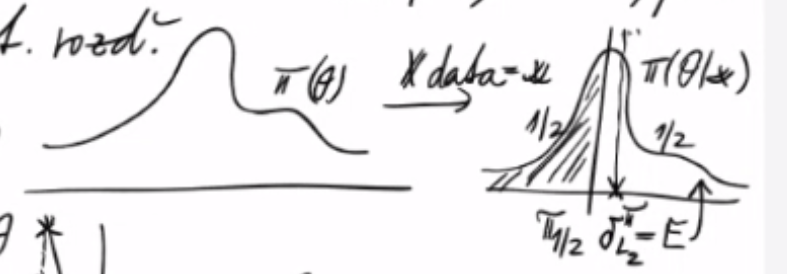
\includegraphics[width=0.7\linewidth]{pictures/10.12}
			\caption{popis}
			\label{fig:10}
		\end{figure}
		\FloatBarrier
\begin{theorem}\label{veta7}
$f,~\pi,~L=L_{k_1,k_2}(\t,\delta)=\begin{cases}
		k_1(\delta-\t)&\delta\geq \t \\ k_2(\t-\delta)& \delta<\t.
		\end{cases}$ (multilineární loss). Nechť $0<\E\big(|\t|\big|\textbf{x}\big)<+\infty$. Pak $\delta^\pi(\textbf{x})=\pi_{\frac{k_2}{k_1+k_2}}(\t|\textbf{x})$, kde $\frac{k_2}{k_1+k_2}$ je kvantil aposteriorního rozdělení.		
		\begin{proof}
		Spočítáme si, jak vypadá aposteriorní bayesovské riziko:
			\[
			\begin{split}
			\rho(\pi,&\delta|\textbf{x})=\E^{\pi}\big[L_{k_1,k_2}(\t,\delta)\big| \textbf{x}\big]=k_1\int_{-\infty}^\delta (\delta-\t)\pi(\t|\textbf{x})\d\t+k_2\int_\delta^{+\infty}(\t-\delta)\pi(\t|\textbf{x})\d\t\stackrel{P.P.}{=}\\
			&=k_1\Big(\big[(\delta-\t)\FF_\pi(\t|\textbf{x})\big]_{-\infty}^\delta+\int_{-\infty}^\delta \FF_\pi(\t|\textbf{x})\d\t\Big)+k_2\cdot (\dots)=\\
			&=k_1\Big( 0-\underbrace{\delta\cdot\FF_\pi(-\infty|\textbf{x})}_{0}+\underbrace{\lim\limits_{\t\to-\infty}\t\FF_\pi(\t|\textbf{x})}_{0\text{, protože }\int_\Theta |\t|\pi(\t|\textbf{x})<\infty}+\int_{-\infty}^\delta \FF_\pi(\t|\textbf{x})\d\t \Big)+k_2\cdot (\dots\text{\footnotemark})=\\
			&=k_1\int_{-\infty}^\delta \FF_\pi(\t|\textbf{x})\d\t+k_2\int_\delta^{+\infty}\big(1-\FF_\pi(\t|\textbf{x})\big)\d\t.
			\end{split}
			\]
			\[
			\begin{split}
			\rho_\delta'&=k_1\cdot 1\cdot\FF_\pi(\delta|\textbf{x})+k_2\cdot(-1)\big(1-\FF_\pi(\delta|\textbf{x})\big)=0,\\
			\FF_\pi(\delta|\textbf{x})&=\frac{k_2}{k_1+k_2}\in(0,1)\Rightarrow \delta(\textbf{x})=\pi_{\frac{k_2}{k_1+k_2}}(\t|\textbf{x})
			\end{split}
			\]
			\footnotetext{$0=\lim\limits_{\t\to+\infty}\t(1-\FF_{\pi}(\t|\textbf{x}))$}
		\end{proof} 

	
\end{theorem}
\begin{theorem}
	Mějme $f,~\pi,~L=L_{\{0,1\}}(\t,\delta)\equal{ozn}L_{0,1}(\t,\delta)=\begin{cases}
	0&|\t-\delta|\leq c,\\1& |\t-\delta|>c.
	\end{cases}$. Pak Bayesovské řešení $\delta^\pi(\textbf{x})$ je středem intervalu $I_{2c}$ délky $2c$, který maximalizuje $\PP^\pi(\t\in I_{2c}|\textbf{x})$.
	\begin{proof}
		Přenecháno čtenáři (Zkouškový důkaz).
		
		Nápověda: Vyjít z $\rho(\pi,\delta(\textbf{x})|\textbf{x})$ a vyrobit tam $\argmin \rho$.
	\end{proof}
\begin{figure}[h]
	\centering
	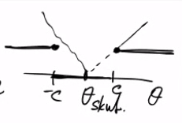
\includegraphics[width=0.7\linewidth]{pictures/10.12-2}
	\caption{popis}
	\label{fig:105}
\end{figure}
\end{theorem}
\FloatBarrier

\begin{define}
	Definujeme \textbf{maximum aposteriori odhad rozhodovací funkce} (někdy také Bayesovská maximálně věrohodný odhad) vztahem $\delta_\mathrm{MAP}(\textbf{x})=\argmax_\t \underbrace{\pi(\t|\textbf{x})}_{\frac{f\cdot\pi}{\int f\cdot\pi\,\d\t}}$ nebo alternativně, pokud $\int f\cdot\pi\,\d\t=+\infty$, definujeme vztahem  $\delta_\mathrm{MAP}(\textbf{x})=\argmax_\t f(\textbf{x}|\t)\pi(\t).$
\end{define}

\begin{example}
$\N(\mu,\sigma^2)$
\begin{enumerate}[a)]
\item $\sigma^2$ známé $\Rightarrow$ $\widehat{\mu}_{MAP}=?$ při $\pi(\mu)=konst.$
\item $\mu$ známé $\Rightarrow$ $\widehat{\sigma}_{MAP}=?$ při $\pi(\sigma)=\frac{1}{\sigma}$ (tzn. $\pi(\log \sigma)=konst.$)
\item $\mu$ i $\sigma^2$ neznámá $\Rightarrow$ $(\widehat{\mu}_{MAP},\widehat{\sigma}_{MAP})$ 2D Bayesovský maximálně věrohodný odhad (MAP)
\end{enumerate}
\end{example}

\chapter{Vzorkování podle důležitosti, Metropolisův algoritmus, variační Bayes.}

\includepdf[pages=-]{scan.pdf}

